% This LaTeX document needs to be compiled with XeLaTeX.
\documentclass[10pt]{article}
\usepackage[utf8]{inputenc}
\usepackage{amsmath}
\usepackage{amsfonts}
\usepackage{amssymb}
\usepackage[version=4]{mhchem}
\usepackage{stmaryrd}
\usepackage{graphicx}
\usepackage[export]{adjustbox}
\graphicspath{ {./images/} }
\usepackage{bbold}
\usepackage{arydshln}
\usepackage[fallback]{xeCJK}
\usepackage{polyglossia}
\usepackage{fontspec}
\IfFontExistsTF{Noto Serif CJK TC}
{\setCJKmainfont{Noto Serif CJK TC}}
{\IfFontExistsTF{STSong}
  {\setCJKmainfont{STSong}}
  {\IfFontExistsTF{Droid Sans Fallback}
    {\setCJKmainfont{Droid Sans Fallback}}
    {\setCJKmainfont{SimSun}}
}}

\setmainlanguage{spanish}
\IfFontExistsTF{CMU Serif}
{\setmainfont{CMU Serif}}
{\IfFontExistsTF{DejaVu Sans}
  {\setmainfont{DejaVu Sans}}
  {\setmainfont{Georgia}}
}

\begin{document}
\section*{Capítulo 4}
\section*{Flujo de mínimo costo}
\section*{1. Introducción.}
Sea $G=(V, E)$ un grafo dirigido. Supongamos que cada rama $e \in E$ tiene asignada una capacidad $u_{e}$, $0<u_{e} \leq \infty$ y un costo $c_{e}$ y que cada vértice $v$ tiene asignado un número real $b_{v}$. Supondremos además que $\sum_{v} b_{v}=0$. Queremos encontrar un flujo $x=\left(x_{e}\right)$ tal que

$$
\begin{aligned}
& x(v, V)-x(V, v)=b_{v} \quad \forall v \in V \\
& 0 \leq x_{e} \leq u_{e} \quad \forall e \in E
\end{aligned}
$$

y de manera que $\sum_{e \in E} c_{e} x_{e}$ sea mínimo. En otras palabras, queremos resolver el problema de programación lineal

$$
\begin{gathered}
\min \sum_{(v, w) \in E} c_{v w} x_{v w} \\
\sum_{w /(v, w) \in E} x_{v w}-\sum_{w /(w, v) \in E} x_{w v}=b_{v} \quad \forall v \in V \\
0 \leq x_{v w} \leq u_{v w} \quad \forall(v, w) \in E
\end{gathered}
$$

Notemos que la condición $\sum_{v} b_{v}=0$ es necesaria para que exista una solución factible del problema ya que si $x$ es una solución factible entonces debe satisfacerse

$$
0=x(V, V)-x(V, V)=\sum_{v} x(v, V)-\sum_{v} x(V, v)=\sum_{v}(x(v, V)-x(V, v))=\sum_{v} b_{v}
$$

Si $b_{v}>0$ llamaremos a $b_{v}$ la oferta del vértice $v$, si $b_{v}=0$ diremos que $v$ es un punto de transferencia y si $b_{v}<0$ llamaremos a $-b_{v}$ la demanda del vértice $v$. Sea $A$ la matriz de incidencia vértice-rama de $G$, es decir, la matriz que tiene una fila para cada vértice $v$ y una columna para cada rama $e$ y cuyos coeficientes están dados por

$$
a_{v e}= \begin{cases}1 & \text { si } v \text { es la cola de } e \\ -1 & \text { si } v \text { es la punta de } e \\ 0 & \text { en otro caso }\end{cases}
$$

Tomemos las coordenadas de $x=\left(x_{e}\right)_{e \in E}, c=\left(c_{e}\right)_{e \in E}$ y $u=\left(u_{e}\right)_{e \in E}$ en el mismo orden que las columnas de $A$. Entonces podemos escribir $c x$ en lugar de $\sum_{e} c_{e} x_{e}$ y $x \leq u$ en lugar de $x_{e} \leq u_{e}(e \in E)$. Además, la $v$-ésima ecuación del sistema $A x=b$ resulta ser

$$
x(v, V)-x(V, v)=b_{v}
$$

En efecto, como $a_{v e}=0,1,-1$,

$$
\left\{e \in E / a_{v e}=1\right\}=\{e \in E / v \text { es la cola de } e\}=\{(v, w) \in E / w \in V\}
$$

y

$$
\left\{e \in E / a_{v e}=-1\right\}=\{e / v \text { es la punta de } e\}=\{(w, v) \in E / w \in V\}
$$

entonces la fila $v$ de $A x$ es

$$
\begin{aligned}
& \sum_{e} a_{v e} x_{e}=\sum_{e / a_{v e}=1} x_{e}-\sum_{e / a_{v e}=-1} x_{e}= \\
= & \sum_{w /(v, w) \in E} x_{v w}-\sum_{w /(w, v) \in E} x_{w v}=x(v, V)-x(V, v)
\end{aligned}
$$

Luego, podemos escribir el problema en la forma

$$
\begin{aligned}
& \min c x \\
& A x=b \\
& 0 \leq x \leq u
\end{aligned}
$$

Ejemplo 1.1. Consideremos el grafo dirigido\\
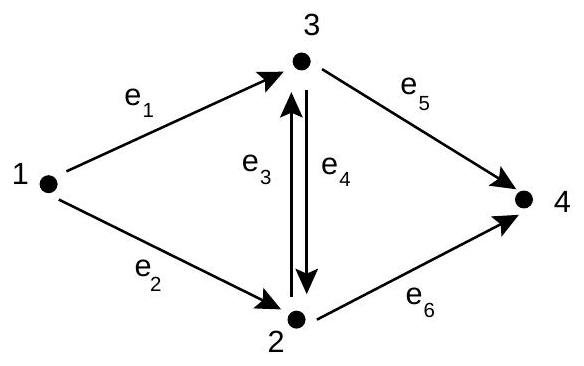
\includegraphics[max width=\textwidth, center]{2025_09_05_955b52bfc43174a24a9ag-02}

Sea $b=\left(b_{1}, b_{2}, b_{3}, b_{4}\right)$. Entonces, si elegimos el orden $(1,3),(1,2),(3,2),(2,3),(3,4),(2,4)$ para las columnas de $A$ la matriz de incidencia vértice-rama es

$$
A=\left(\begin{array}{cccccc}
1 & 1 & 0 & 0 & 0 & 0 \\
0 & -1 & -1 & 1 & 0 & 1 \\
-1 & 0 & 1 & -1 & 1 & 0 \\
0 & 0 & 0 & 0 & -1 & -1
\end{array}\right)
$$

Tomando $x=\left(x_{13}, x_{12}, x_{32}, x_{23}, x_{34}, x_{24}\right)$ entonces el sistema $A x=b$ es

$$
\left(\begin{array}{cccccc}
1 & 1 & 0 & 0 & 0 & 0 \\
0 & -1 & -1 & 1 & 0 & 1 \\
-1 & 0 & 1 & -1 & 1 & 0 \\
0 & 0 & 0 & 0 & -1 & -1
\end{array}\right) \cdot\left(\begin{array}{c}
x_{13} \\
x_{12} \\
x_{32} \\
x_{23} \\
x_{34} \\
x_{24}
\end{array}\right)=\left(\begin{array}{c}
b_{1} \\
b_{2} \\
b_{3} \\
b_{4}
\end{array}\right)
$$

es decir,

$$
\begin{aligned}
x_{13}+x_{12} & =b_{1} \\
-x_{12}-x_{32}+x_{23}+x_{24} & =b_{2} \\
-x_{13}+x_{32}-x_{23}+x_{34} & =b_{3} \\
-x_{34}-x_{24} & =b_{4}
\end{aligned}
$$

que es el sistema

$$
\begin{aligned}
& x(1, V)-x(V, 1)=b_{1} \\
& x(2, V)-x(V, 2)=b_{2} \\
& x(3, V)-x(V, 3)=b_{3} \\
& x(3, V)-x(V, 3)=b_{4}
\end{aligned}
$$

Observación 1.2. Sea $A \in \mathbb{R}^{m \times n}$ una matriz que tiene $n$ columnas distintas tales que en en cada una de ellas hay un solo 1 , un solo -1 y los restantes coeficientes son nulos. Entonces existe un grafo dirigido $G$ con $m$ vértices y $n$ ramas tal que $A$ es la matriz de incidencia vértice-rama de $G$. Por ejemplo

$$
A=\left(\begin{array}{ccccc}
1 & 0 & 0 & -1 & 1 \\
0 & -1 & 0 & 0 & -1 \\
-1 & 0 & 1 & 0 & 0 \\
0 & 1 & -1 & 1 & 1
\end{array}\right)
$$

es la matriz de incidencia vértice-rama del grafo\\
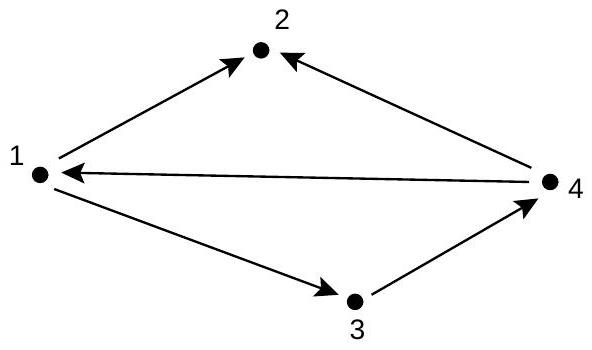
\includegraphics[max width=\textwidth, center]{2025_09_05_955b52bfc43174a24a9ag-03}

Además, si $A \in R^{m \times n}$ es una matriz de coeficientes ceros y unos tal que en cada columna los unos aparecen en forma consecutiva y $b$ es un vector cualquiera de $\mathbb{R}^{m}$ entonces el sistema $A x=b$ es equivalente al sistema $A^{\prime} x=b^{\prime}$, donde $\left[A^{\prime} \mid b^{\prime}\right]$ se obtiene de $[A \mid b]$ haciendo la transformación de filas

$$
F_{1}^{\prime}=F_{1}, F_{2}^{\prime}=F_{2}-F_{1}, F_{3}^{\prime}=F_{3}-F_{2}, \ldots, F_{m}^{\prime}=F_{m}-F_{m-1}, F_{m+1}^{\prime}=-F_{m}
$$

y se verifica que $A^{\prime} \in \mathbb{R}^{(m+1) \times n}$ tiene en cada columna un solo 1 , un solo - 1 y los restantes coeficientes nulos, es decir, es una matriz de incidencia vértice-rama de algún grafo con $m+1$ vértices y $n$ ramas y $b^{\prime} \in \mathbb{R}^{m+1}$ verifica $\sum_{i=1}^{m+1} b_{i}^{\prime}=0$. Por ejemplo, si

$$
[A \mid b]=\left(\begin{array}{ccccc|c}
1 & 1 & 1 & 0 & 0 & 1 \\
0 & 1 & 1 & 1 & 1 & 5 \\
0 & 0 & 1 & 0 & 1 & -1
\end{array}\right)
$$

entonces

$$
\left[A^{\prime} \mid b^{\prime}\right]=\left(\begin{array}{ccccc:c}
1 & 1 & 1 & 0 & 0 & 1 \\
-1 & 0 & 0 & 1 & 1 & 4 \\
0 & -1 & 0 & -1 & 0 & -6 \\
0 & 0 & -1 & 0 & -1 & 1
\end{array}\right)
$$

Esto significa que si $A$ es una matriz que tiene en cada columna un solo 1 , un solo -1 y los restantes coeficientes nulos y $b$ es un vector tal que la suma de sus coordenadas es cero o si $A$ es una matriz de coeficientes ceros y unos tal que en cada columna los unos aparecen en forma consecutiva y $b$ es un vector cualquiera entonces, dados $c$ y $u$, el problema

$$
\begin{aligned}
& \min c x \\
& A x=b \\
& 0 \leq x \leq u
\end{aligned}
$$

puede expresarse como un problema de flujo de mínimo costo en algún grafo $G$.\\
Ejemplo 1.3. Las fábricas 1 y 2 producen 80 y 70 unidades de un cierto producto que deben ser transportadas a los depósitos 3 y 4, los que demandan 60 y 90 unidades respectivamente. El transporte puede\\
realizarse en forma directa por tren, con capacidad ilimitada, o por camión, en cuyo caso debe pasarse necesariamente por un centro de distribución 5 y no pueden transportarse más de 50 unidades por vez. Sea $c_{i j}$ el costo de transportar una unidad de $i$ a $j$ y sea $x_{i j}$ la cantidad de unidades que deben transportarse de $i$ a $j$. Queremos determinar cuánto debe valer $x=\left(x_{i j}\right)$ de manera tal que el costo del transporte sea mínimo. Podemos representar la situación en el grafo\\
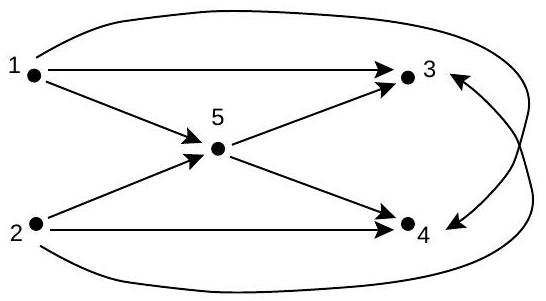
\includegraphics[max width=\textwidth, center]{2025_09_05_955b52bfc43174a24a9ag-04}\\
donde asignamos capacidad infinita a las ramas $(1,3),(1,4),(2,3)$ y $(2,4)$ (transporte por tren) y capacidad 50 a las restantes ramas (transporte en camión).\\
Sean $b=(80,70,-60,-90,0), u_{13}=u_{14}=u_{23}=u_{24}=\infty \mathrm{y} u_{15}=u_{53}=u_{25}=u_{54}=50$. Entonces el problema puede escribirse

$$
\begin{aligned}
& \min \sum_{e \in E} c_{e} x_{e} \\
& x(i, V)-x(V, i)=b_{i} \quad \forall i \in V \\
& 0 \leq x_{e} \leq u_{e} \quad \forall e \in E
\end{aligned}
$$

Luego, este es un ejemplo de un problema de flujo de mínimo costo.\\
Ejemplo 1.4. El problema del transporte que vimos en el capítulo 3 es un problema de flujo de mínimo costo. En efecto, el problema

$$
\begin{aligned}
& \min \sum_{i, j} c_{i j} x_{i j} \\
& \sum_{j=1}^{n} x_{i j}=a_{i} \quad(1 \leq i \leq m) \\
& \sum_{i=1}^{m} x_{i j}=b_{j} \quad(1 \leq j \leq n) \\
& x_{i j} \geq 0 \quad \forall i, j
\end{aligned}
$$

donde se supone que $\sum_{i=1}^{m} a_{i}=\sum_{j=1}^{n} b_{j}$, puede escribirse

$$
\begin{aligned}
& \min \sum_{i, j} c_{i j} x_{i j} \\
& \sum_{j=1}^{n} x_{i j}=a_{i} \quad(1 \leq i \leq m) \\
& -\sum_{i=1}^{m} x_{i j}=-b_{j} \quad(1 \leq j \leq n) \\
& x_{i j} \geq 0 \quad \forall i, j
\end{aligned}
$$

donde se verifica $\sum_{i=1}^{m} a_{i}+\sum_{i=1}^{n}-b_{i}=0$.

Sea $G=(V, E)$ el grafo definido por $V=\left\{d_{1}, d_{2}, \ldots, d_{m}, l_{1}, l_{2}, \ldots, l_{n}\right\}$ (un vértice para cada depósito y cada localidad) y $E=\left\{\left(d_{i}, l_{j}\right) / 1 \leq i \leq m, \quad 1 \leq j \leq n\right\}$ y sea $\left(a_{1}, \ldots, a_{m},-b_{1}, \ldots,-b_{n}\right)$ el vector que representa la oferta y la demanda, cuyas coordenadas suman cero. Sea $x_{i j}$ el flujo de la rama ( $d_{i}, l_{j}$ ). Como

$$
\begin{aligned}
& x\left(d_{i}, V\right)=\sum_{j=1}^{n} x_{i j} \\
& x\left(V, d_{i}\right)=0 \\
& x\left(l_{j}, V\right)=0 \\
& x\left(V, l_{j}\right)=\sum_{i=1}^{m} x_{i j}
\end{aligned}
$$

las ecuaciones

$$
\begin{aligned}
& \sum_{j=1}^{n} x_{i j}=a_{i} \quad(1 \leq i \leq m) \\
& -\sum_{i=1}^{m} x_{i j}=-b_{j} \quad(1 \leq j \leq n)
\end{aligned}
$$

se escriben

$$
\begin{aligned}
x\left(d_{i}, V\right)-x\left(V, d_{i}\right) & =a_{i} \quad(1 \leq i \leq m) \\
x\left(l_{j}, V\right)-x\left(V, l_{j}\right) & =-b_{j} \quad(1 \leq j \leq n)
\end{aligned}
$$

Esto muestra que el problema del transporte es un problema de flujo de mínimo costo.\\
Ejemplo 1.5. Un avión recorre las ciudades $1,2,3$ y 4 en ese orden. Para cada $i<j$ sea $u_{i j}$ el número de personas que desean viajar de $i$ a $j$ y sea $c_{i j}$ el costo del pasaje de $i$ a $j$. Sea $r$ el número de pasajeros que caben en el avión. El objetivo es determinar la cantidad de pasajes $x_{i j}$ de $i$ a $j$ que conviene vender de manera que $\sum c_{i j} x_{i j}$ sea máximo, es decir, tal que $\sum\left(-c_{i j}\right) x_{i j}$ sea mínimo sujeto a las restricciones

$$
\begin{aligned}
x_{12}+x_{13}+x_{14} & \leq r \\
x_{13}+x_{14}+x_{23}+x_{24} & \leq r \\
x_{14}+x_{24}+x_{34} & \leq r \\
0 \leq x_{i j} \leq u_{i j} &
\end{aligned}
$$

(al partir de cada ciudad la cantidad de pasajeros a bordo del avión debe ser a lo sumo $r$ ).\\
Agregando a cada desigualdad una variable de holgura podemos escribir las restricciones en la forma

$$
\begin{gathered}
x_{12}+x_{13}+x_{14}+s_{1}=r \\
x_{13}+x_{14}+x_{23}+x_{24}+s_{2}=r \\
x_{14}+x_{24}+x_{34}+s_{3}=r \\
0 \leq x_{i j} \leq u_{i j} \\
0 \leq s_{i}
\end{gathered} \quad
$$

Escribimos el sistema

$$
\begin{aligned}
x_{12}+x_{13}+x_{14}+s_{1} & =r \\
x_{13}+x_{14}+x_{23}+x_{24}+s_{2} & =r \\
x_{14}+x_{24}+x_{34}+s_{3} & =r
\end{aligned}
$$

en la forma $A x=b$, donde

$$
[A \mid b]=\left(\begin{array}{ccccccccc:c}
1 & 1 & 1 & 0 & 0 & 0 & 1 & 0 & 0 & r \\
0 & 1 & 1 & 1 & 1 & 0 & 0 & 1 & 0 & r \\
0 & 0 & 1 & 0 & 1 & 1 & 0 & 0 & 1 & r
\end{array}\right)
$$

y $x=\left(x_{12}, x_{13}, x_{14}, x_{23}, x_{24}, x_{34}, s_{1}, s_{2}, s_{3}\right)$. Como $A$ es una matriz de coeficientes ceros y unos tal que en cada columna los unos aparecen en forma consecutiva, aplicando la transformación de filas

$$
F_{1}^{\prime}=F_{1}, F_{2}^{\prime}=F_{2}-F_{1}, F_{3}^{\prime}=F_{3}-F_{2}, F_{4}^{\prime}=-F_{3}
$$

(ver observación 1.2.) obtenemos el sistema equivalente $A^{\prime} x=b^{\prime}$ donde

$$
\left[A^{\prime} \mid b^{\prime}\right]=\left(\begin{array}{ccccccccc:c}
1 & 1 & 1 & 0 & 0 & 0 & 1 & 0 & 0 & r \\
-1 & 0 & 0 & 1 & 1 & 0 & -1 & 1 & 0 & 0 \\
0 & -1 & 0 & -1 & 0 & 1 & 0 & -1 & 1 & 0 \\
0 & 0 & -1 & 0 & -1 & -1 & 0 & 0 & -1 & -r
\end{array}\right)
$$

Luego, el problema puede escribirse en la forma

$$
\begin{aligned}
& \min c^{\prime} x \\
& A^{\prime} x=b^{\prime} \\
& 0 \leq x \leq u
\end{aligned}
$$

con $u=\left(u_{12}, u_{13}, u_{14}, u_{23}, u_{24}, u_{34}, \infty, \infty, \infty\right)$ (ya que las variables de holgura no tienen restricciones de capacidad), $c^{\prime}=\left(-c_{12},-c_{13},-c_{14},-c_{23},-c_{24},-c_{34}, 0,0,0\right)$ y donde $A^{\prime}$ es una matriz de incidencia vérticerama de algún grafo y la suma de las coordenadas de $b^{\prime}$ es cero. Luego, este problema también puede plantearse como un problema de flujo de mínimo costo.

Ejemplo 1.6. El problema de máximo flujo visto en el capítulo anterior es un caso particular del problema de flujo de mínimo costo. En efecto, agregando al grafo una rama de $t$ a $s$ con capacidad $u_{t s}=\infty$ el problema de máximo flujo puede plantearse en la forma

$$
\begin{aligned}
& \min -x_{t s} \\
& x(v, V)-x(V, v)=0 \quad(v \in V) \\
& 0 \leq x_{e} \leq u_{e}
\end{aligned}
$$

\section*{2. Optimalidad de una solución factible.}
Sea $G=(V, E)$ un grafo dirigido donde cada rama $e$ tiene asignada una capacidad $u_{e}\left(0<u_{e} \leq \infty\right)$ y un costo $c_{e}$ y cada vértice $v$ tiene asignado un número real $b_{v}$. Supongamos además que $\sum_{v} b_{v}=0 \mathrm{y}$ consideremos el problema de hallar un flujo $x$ en $G$ de mínimo costo sujeto a las restricciones

$$
\begin{aligned}
& x(v, V)-x(V, v)=b_{v} \quad \forall v \in V \\
& 0 \leq x_{e} \leq u_{e} \quad \forall e \in E
\end{aligned}
$$

En esta sección hallaremos condiciones necesarias y suficientes para que una solución factible sea óptima. Para ello usaremos el teorema de holgura complementaria (capítulo 1 , teorema 4.9.).

Teorema 2.1. Sea $x$ una solución factible. Entonces $x$ es una solución óptima si y sólo si existe $\left(y_{v}\right)_{v \in V}$ que verifica las dos siguientes condiciones\\
i) $x_{v w}>0 \Longrightarrow c_{v w}+y_{v}-y_{w} \leq 0$\\
ii) $x_{v w}<u_{v w} \Longrightarrow c_{v w}+y_{v}-y_{w} \geq 0$

Demostración: Supongamos primero que $u_{v w}<\infty$ para todo $(v, w) \in E$ y escribamos el problema en la forma


\begin{gather*}
\min c x \\
-A x=-b \\
x \leq u  \tag{1}\\
x \geq 0
\end{gather*}


donde $A$ es la matriz de incidencia vértice-rama de $G$. Agregando una variable de holgura para cada condición $x_{e} \leq u_{e}$, es decir, reemplazando cada condición $x_{e} \leq u_{e}$ por la ecuación $x_{e}+s_{e}=u_{e}$, el problema es equivalente al problema de programación lineal en forma standard


\begin{gather*}
\min (c, 0) \cdot(x, s) \\
\left(\begin{array}{cc}
-A & 0 \\
I & I
\end{array}\right)\binom{x}{s}=\binom{-b}{u}  \tag{P}\\
(x, s) \geq 0
\end{gather*}


donde $I$ es la matriz identidad que tiene una fila y una columna para cada rama $e \in E$. El problema dual, con variables $(y, z)$ es


\begin{align*}
& \max (y, z) \cdot(-b, u) \\
& (y, z) \cdot\left(\begin{array}{cc}
-A & 0 \\
I & I
\end{array}\right) \leq(c, 0) \tag{D}
\end{align*}


es decir,

$$
\begin{gathered}
\max -b y+u z \\
-y A+z I \leq c \\
z I \leq 0
\end{gathered}
$$

Recordemos que $A$ tiene una columna por cada rama de $G$ y que en la columna correspondiente a una rama ( $v, w$ ) los coeficientes de $A$ son todos nulos salvo los correspondientes a las filas $v$ y $w$ que son 1 y - 1 respectivamente. Luego, las restricciones del dual son

$$
\begin{gathered}
-y_{v}+y_{w}+z_{v w} \leq c_{v w} \quad((v, w) \in E) \\
z_{v w} \leq 0 \quad((v, w) \in E)
\end{gathered}
$$

Dado $\left(y_{v}\right)_{v \in V}$, si $\bar{c}_{v w}=c_{v w}+y_{v}-y_{w}((v, w) \in E)$ entonces $(y, z)$ es una solución factible de (D) si y sólo si

$$
\begin{aligned}
& z_{v w} \leq \bar{c}_{v w} \quad((v, w) \in E) \\
& z_{v w} \leq 0 \quad((v, w) \in E)
\end{aligned}
$$

o, equivalentemente,

$$
z_{v w} \leq \min \left\{\bar{c}_{v w}, 0\right\} \quad((v, w) \in E)
$$

Además, si $(y, z)$ es una solución óptima de ( D ) entonces $z_{v w}=\min \left\{\bar{c}_{v w}, 0\right\}$ para todo $(v, w) \in E$. En efecto, supongamos que $z_{v w}<\min \left\{\bar{c}_{v w}, 0\right\}$ para algún $(v, w) \in E$. Sea $\epsilon>0$ tal que $z_{v w}+\epsilon \leq 0$ y $z_{v w}+\epsilon \leq \bar{c}_{v w}$. Sea $z^{\prime}$ el vector definido por

$$
z_{e}^{\prime}= \begin{cases}z_{e} & \text { si } e \neq(v, w) \\ z_{v w}+\epsilon & \text { si } e=(v, w)\end{cases}
$$

Entonces $\left(y, z^{\prime}\right)$ es una solución factible del dual $y-b y+u z^{\prime}=-b y+u z+u_{v w} \cdot \epsilon>-b y+u z$, lo que contradice la optimalidad de $(y, z)$.\\
Ahora estamos en condiciones de probar que si $x$ es una solución factible de (1) entonces $x$ es una solución óptima si y sólo si existe $\left(y_{v}\right)_{v \in V}$ que verifica las condiciones i) y ii).\\
$(\Longrightarrow)$ Supongamos que $x$ es una solución óptima de (1) y sea $s=u-x$ (recordemos que estamos suponiendo que $u_{v w}<\infty$ para todo $\left.(v, w) \in E\right)$. Entonces $(x, s)$ es una solución óptima de $(\mathrm{P})$. Sea $(y, z)$ una solución óptima del dual y sea $\bar{c}_{v w}=c_{v w}+y_{v}-y_{w}$ para cada $(v, w) \in E$. Entonces las condiciones i) y ii) pueden escribirse\\
i) $x_{v w}>0 \Longrightarrow \bar{c}_{v w} \leq 0$\\
ii) $x_{v w}<u_{v w} \Longrightarrow \bar{c}_{v w} \geq 0$

Como $(y, z)$ es una solución óptima de $(\mathrm{D})$ se verifica que $z_{v w}=\min \left\{\bar{c}_{v w}, 0\right\}$ para todo $(v, w) \in E$ y además, por el teorema de holgura complementaria se tiene que

$$
(x, s)\left[(c, 0)-(y, z) \cdot\left(\begin{array}{cc}
-A & 0 \\
I & I
\end{array}\right)\right]=0
$$

Como $A$ tiene una columna por cada rama de $G$ y en la columna correspondiente a una rama ( $v, w$ ) los coeficientes de $A$ son todos nulos salvo los correspondientes a las filas $v$ y $w$ que son 1 y -1 respectivamente, esto es equivalente a

$$
\begin{aligned}
& x_{v w}\left[c_{v w}+y_{v}-y_{w}-z_{v w}\right]=0 \\
& s_{v w} \cdot z_{v w}=0
\end{aligned}
$$

es decir,

$$
\begin{aligned}
& x_{v w}\left[\bar{c}_{v w}-z_{v w}\right]=0 \\
& s_{v w} \cdot z_{v w}=0
\end{aligned}
$$

Luego, si $x_{v w}>0$ entonces $\bar{c}_{v w}=z_{v w}=\min \left\{\bar{c}_{v w}, 0\right\}$ de donde $\bar{c}_{v w} \leq 0$ y si $x_{v w}<u_{v w}$ entonces $s_{v w}>0$ con lo cual $0=z_{v w}=\min \left\{\bar{c}_{v w}, 0\right\}$ de donde $\bar{c}_{v w} \geq 0$, es decir, se satisfacen i) y ii).\\
$(\Longleftarrow)$ Supongamos ahora que existe $\left(y_{v}\right)_{v \in V}$ que verifica i) y ii). Sean $\bar{c}$ y $z$ los vectores definidos por

$$
\begin{aligned}
& \bar{c}_{v w}=c_{v w}+y_{v}-y_{w} \quad((v, w) \in E) \\
& z_{v w}=\min \left\{\bar{c}_{v w}, 0\right\} \quad((v, w) \in E)
\end{aligned}
$$

Entonces $(y, z)$ es una solución factible del dual. Luego, por el teorema de holgura complementaria, para ver que $x$ es óptimo basta mostrar que $(x, s)$ e $(y, z)$ satisfacen la condición de holgura complementaria

$$
(x, s)\left[(c, 0)-(y, z) \cdot\left(\begin{array}{cc}
-A & 0 \\
I & I
\end{array}\right)\right]=0
$$

es decir, satisfacen

$$
\begin{aligned}
& x_{v w}\left[\bar{c}_{v w}-z_{v w}\right]=0 \\
& s_{v w} \cdot z_{v w}=0
\end{aligned}
$$

Si $x_{v w}=0$ entonces claramente se satisface la primera ecuación y, como $x_{v w}=0<u_{v w}$ la condición ii) garantiza que $\bar{c}_{v w} \geq 0$, de donde $z_{v w}=\min \left\{\bar{c}_{v w}, 0\right\}=0$ y por lo tanto también se satisface la segunda ecuación.\\
Si $x_{v w}=u_{v w}$ entonces $s_{v w}=0$ (luego se satisface la segunda ecuación) y como vale $x_{v w}=u_{v w}>0$, por la condición i) resulta que $\bar{c}_{v w} \leq 0$, de donde $z_{v w}=\min \left\{\bar{c}_{v w}, 0\right\}=\bar{c}_{v w}$ y por lo tanto también se satisface la primera ecuación.\\
Por último, si $0<x_{v w}<u_{v w}$ entonces por i) y ii) resulta que $\bar{c}_{v w}=0$ con lo cual $z_{v w}=\min \left\{\bar{c}_{v w}, 0\right\}=0 \mathrm{y}$ por lo tanto también en este caso se satisfacen ambas ecuaciones.

Ahora supongamos que $u_{v w}=\infty$ para algunos $(v, w) \in E$.

Sea $\mathcal{L}=\left\{(v, w) \in E / u_{v w}=\infty\right\}$. Entonces las condiciones $x_{v w} \leq u_{v w}$ en (1) son superfluas para $(v, w) \in \mathcal{L}$ y no tiene sentido agregar variables de holgura para ellas. En este caso (1) es equivalente a

$$
\begin{gathered}
\min c x \\
-A x=-b \\
x \leq u \quad(e \in E-\mathcal{L}) \\
x \geq 0
\end{gathered}
$$

Sea $n=\# E$ y sea $k=\#(E-\mathcal{L})$. Ahora, agregando una variable de holgura para cada una de las $k$ condiciones $x_{e} \leq u_{e}(e \in E-\mathcal{L})$, es decir, reemplazando cada una de estas condiciones por la igualdad $x_{e}+s_{e}=u_{e}$, el problema es equivalente a


\begin{gather*}
\min (c, 0) \cdot(x, s) \\
\left(\begin{array}{cc}
-A & 0 \\
I^{\prime} & I_{k}
\end{array}\right)\binom{x}{s}=\binom{-b}{u^{\prime}}  \tag{$\prime$}\\
(x, s) \geq 0
\end{gather*}


donde $I^{\prime}$ tiene una fila por cada rama $e \in E-\mathcal{L}$, una columna por cada rama $e \in E$ y es la matriz que resulta de eliminar en $I$ las filas correspondientes a las ramas $e \in \mathcal{L}$ (donde $I$ es la matriz identidad que tiene una fila y una columna por cada rama $e \in E$ ), el vector $u^{\prime}$ resulta de eliminar en $u$ las coordenadas $u_{e}$ ( $e \in \mathcal{L}$ ) y la matriz $I_{k}$ es la matriz identidad que tiene una fila y una columna por cada rama de capacidad finita, es decir, por cada una de las $k$ ramas de $E-\mathcal{L}$.\\
Por ejemplo, si el grafo es\\
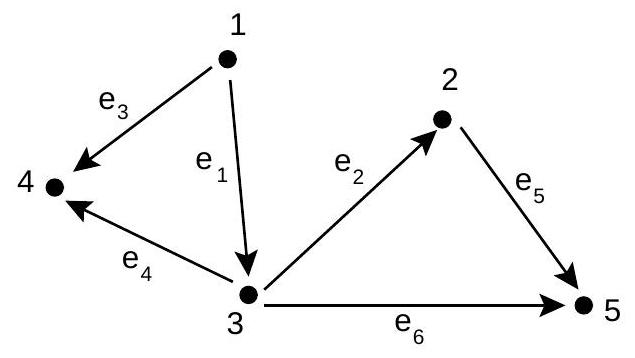
\includegraphics[max width=\textwidth, center]{2025_09_05_955b52bfc43174a24a9ag-09}\\
y $e_{1}, e_{3}, e_{5}$ y $e_{6}$ son las ramas de capacidad finita (es decir, $\mathcal{L}=\left\{e_{2}, e_{4}\right\}$ ) entonces agregando una variable de holgura para cada rama $e \notin \mathcal{L}$ el problema puede plantearse en la forma

$$
\begin{gathered}
\min \sum_{i=1}^{6} c_{e_{i}} x_{e_{i}}+0 . s_{e_{1}}+0 . s_{e_{3}}+0 . s_{e_{5}}+0 . s_{e_{6}} \\
-\left(\begin{array}{cccccc}
1 & 0 & 1 & 0 & 0 & 0 \\
0 & -1 & 0 & 0 & 1 & 0 \\
-1 & 1 & 0 & 1 & 0 & 1 \\
0 & 0 & -1 & -1 & 0 & 0 \\
0 & 0 & 0 & 0 & -1 & -1
\end{array}\right) \cdot\left(\begin{array}{l}
x_{e_{1}} \\
x_{e_{2}} \\
x_{e_{3}} \\
x_{e_{4}} \\
x_{e_{5}} \\
x_{e_{6}}
\end{array}\right)=-\left(\begin{array}{l}
b_{1} \\
b_{2} \\
b_{3} \\
b_{4} \\
b_{5}
\end{array}\right) \\
x_{e_{1}}+s_{e_{1}}=u_{e_{1}} \\
x_{e_{3}}+s_{e_{3}}=u_{e_{3}} \\
x_{e_{5}}+s_{e_{5}}=u_{e_{5}} \\
x_{e_{6}}+s_{e_{6}}=u_{e_{6}} \\
x_{e} \geq 0 \quad(e \in E) \\
s_{e} \geq 0 \quad(e \in E-\mathcal{L})
\end{gathered}
$$

lo que puede escribirse

$$
\begin{gathered}
\min \sum_{i=1}^{6} c_{e_{i}} x_{e_{i}}+0 . s_{e_{1}}+0 . s_{e_{3}}+0 . s_{e_{5}}+0 . s_{e_{6}} \\
\left(\begin{array}{cccccc:cccc}
-1 & 0 & -1 & 0 & 0 & 0 & 0 & 0 & 0 & 0 \\
0 & 1 & 0 & 0 & -1 & 0 & 0 & 0 & 0 & 0 \\
1 & -1 & 0 & -1 & 0 & -1 & 0 & 0 & 0 & 0 \\
0 & 0 & 1 & 1 & 0 & 0 & 0 & 0 & 0 & 0 \\
0 & 0 & 0 & 0 & 1 & 1 & 0 & 0 & 0 & 0 \\
- & - & - & - & - & - & - & - & - & - \\
1 & 0 & 0 & 0 & 0 & 0 & 1 & 0 & 0 & 0 \\
0 & 0 & 1 & 0 & 0 & 0 & 0 & 1 & 0 & 0 \\
0 & 0 & 0 & 0 & 1 & 0 & 0 & 0 & 1 & 0 \\
0 & 0 & 0 & 0 & 0 & 1 & 0 & 0 & 0 & 1
\end{array}\right) \cdot\left(\begin{array}{l}
x_{e_{1}} \\
x_{e_{2}} \\
x_{e_{3}} \\
x_{e_{4}} \\
x_{e_{5}} \\
x_{e_{6}} \\
s_{e_{1}} \\
s_{e_{3}} \\
s_{e_{5}} \\
s_{e_{6}}
\end{array}\right)=\left(\begin{array}{c}
-b_{1} \\
-b_{2} \\
-b_{3} \\
-b_{4} \\
-b_{5} \\
u_{e_{1}} \\
u_{e_{3}} \\
u_{e_{5}} \\
u_{e_{6}}
\end{array}\right) \\
s_{e} \geq 0 \\
(e \in E) \\
(e \in E-\mathcal{L})
\end{gathered}
$$

es decir,

$$
\begin{gathered}
\min (c, 0) \cdot(x, s) \\
\left(\begin{array}{cc}
-A & 0 \\
I^{\prime} & I_{k}
\end{array}\right)\binom{x}{s}=\binom{-b}{u^{\prime}} \\
(x, s) \geq 0
\end{gathered}
$$

donde

$$
A=\left(\begin{array}{cccccc}
1 & 0 & 1 & 0 & 0 & 0 \\
0 & -1 & 0 & 0 & 1 & 0 \\
-1 & 1 & 0 & 1 & 0 & 1 \\
0 & 0 & -1 & -1 & 0 & 0 \\
0 & 0 & 0 & 0 & -1 & -1
\end{array}\right)
$$

es la matriz de incidencia vértice-rama de $G$,

$$
I^{\prime}=\left(\begin{array}{cccccc}
1 & 0 & 0 & 0 & 0 & 0 \\
0 & 0 & 1 & 0 & 0 & 0 \\
0 & 0 & 0 & 0 & 1 & 0 \\
0 & 0 & 0 & 0 & 0 & 1
\end{array}\right)
$$

es la matriz que se obtiene eliminando en la matriz identidad que tiene una fila y una columna por cada rama de $G$

$$
I=\left(\begin{array}{llllll}
1 & 0 & 0 & 0 & 0 & 0 \\
0 & 1 & 0 & 0 & 0 & 0 \\
0 & 0 & 1 & 0 & 0 & 0 \\
0 & 0 & 0 & 1 & 0 & 0 \\
0 & 0 & 0 & 0 & 1 & 0 \\
0 & 0 & 0 & 0 & 0 & 1
\end{array}\right)
$$

la segunda y la cuarta fila, es decir, las filas correspondientes a las ramas de capacidad infinita, que en este caso son $e_{2}$ y $e_{4}, I_{k}=I_{4}$ es la matriz identidad y $u^{\prime}=\left(u_{e_{1}}, u_{e_{3}}, u_{e_{5}}, u_{e_{6}}\right)$.\\
Ahora la variable del dual $(y, z)$ es tal que $y$ tiene una coordenada por cada vértice de $G$ y $z$ tiene una coordenada por cada rama de $E-\mathcal{L}$ y las restricciones del dual son

$$
\begin{array}{cc}
-y_{v}+y_{w}+z_{v w} \leq c_{v w} & ((v, w) \in E-\mathcal{L}) \\
-y_{v}+y_{w} \leq c_{v w} & ((v, w) \in \mathcal{L}) \\
z_{v w} \leq 0 & ((v, w) \in E-\mathcal{L})
\end{array}
$$

es decir,

$$
\begin{aligned}
& z_{v w} \leq \min \left\{\bar{c}_{v w}, 0\right\} \quad((v, w) \in E-\mathcal{L}) \\
& \quad \bar{c}_{v w} \geq 0 \quad((v, w) \in \mathcal{L})
\end{aligned}
$$

donde $\bar{c}_{v w}=c_{v w}+y_{v}-u_{w} \mathrm{y}$ vale\\
Si $(y, z)$ es una solución óptima del dual entonces $z_{v w}=\min \left\{\bar{c}_{v w}, 0\right\}$ para toda rama $(v, w) \in E-\mathcal{L}$ y $\bar{c}_{v w} \geq 0$ para toda rama $(v, w) \in \mathcal{L}$.\\
$(\Longrightarrow)$ Supongamos que $x$ es una solución óptima de (1) y, para cada $e \in E-\mathcal{L}$, sea $s_{e}=u_{e}-x_{e}$. Entonces $(x, s)$ es óptimo de ( $\mathrm{P}^{\prime}$ ). Si ( $y, z$ ) es una solución óptima del dual entonces se verifican las condiciones de holgura complementaria, que en este caso son

$$
\begin{aligned}
& x_{v w}\left[\bar{c}_{v w}-z_{v w}\right]=0 \quad((v, w) \in E-\mathcal{L}) \\
& x_{v w} \cdot \bar{c}_{v w}=0 \quad((v, w) \in \mathcal{L}) \\
& s_{v w} \cdot z_{v w}=0 \quad((v, w) \in E-\mathcal{L})
\end{aligned}
$$

Verifiquemos que esto implica que valen las condiciones i) y ii):\\
i) si $x_{v w}>0$ entonces $\bar{c}_{v w} \leq 0$ (para $(v, w) \in E-\mathcal{L}$ la demostración es la misma que en el caso en que todas las capacidades eran finitas y para $(v, w) \in \mathcal{L}$ vale porque de la segunda ecuación resulta que $\bar{c}_{v w}=0$ ).\\
ii) si $x_{v w}<u_{v w}$ entonces $\bar{c}_{v w} \geq 0$ (para $(v, w) \in \mathcal{L}$ vale ya que $(y, z)$ es una solución factible del dual cuyas restricciones son

$$
\begin{gathered}
z_{v w} \leq \min \left\{\bar{c}_{v w}, 0\right\} \quad((v, w) \in E-\mathcal{L}) \\
\quad \bar{c}_{v w} \geq 0 \quad((v, w) \in \mathcal{L})
\end{gathered}
$$

y para $(v, w) \in E-\mathcal{L}$ la demostración es igual que en el caso $u<\infty)$.\\
$(\Longleftarrow)$ Supongamos ahora que existe $\left(y_{v}\right)_{v \in V}$ que verifica i) y ii). Sean $\bar{c}$ y $z$ los vectores definidos por

$$
\begin{aligned}
& \bar{c}_{v w}=c_{v w}+y_{v}-y_{w} \quad((v, w) \in E) \\
& z_{v w}=\min \left\{\bar{c}_{v w}, 0\right\} \quad((v, w) \in E-\mathcal{L})
\end{aligned}
$$

Luego $(y, z)$ es una solución factible del dual (ya que si $(v, w) \in \mathcal{L}$ entonces $x_{v w}<u_{v w}$ de donde $\bar{c}_{v w} \geq 0$ ). Entonces, por el teorema de holgura complementaria, para ver que $x$ es óptimo basta mostrar que $(x, s)$ e ( $y, z$ ) satisfacen las condiciones de holgura complementaria

$$
\begin{aligned}
& x_{v w}\left[\bar{c}_{v w}-z_{v w}\right]=0 \quad((v, w) \in E-\mathcal{L}) \\
& x_{v w} \cdot \bar{c}_{v w}=0 \quad((v, w) \in \mathcal{L}) \\
& s_{v w} \cdot z_{v w}=0 \quad((v, w) \in E-\mathcal{L})
\end{aligned}
$$

La validez de la primera y tercera ecuación se prueba de la misma manera que en el caso $u<\infty$.\\
Para la segunda basta ver que si $x_{v w}>0, \operatorname{con}(v, w) \in \mathcal{L}$, entonces $\bar{c}_{v w}=0$ : si $x_{v w}>0$ entonces, por i), se tiene que $\bar{c}_{v w} \leq 0 \mathrm{y}$ como $(v, w) \in \mathcal{L}$ entonces $u_{v w}=\infty$ de donde $x_{v w}<u_{v w}$. Luego, por ii), $\bar{c}_{v w} \geq 0$. Por lo tanto, $\bar{c}_{v w}=0$.

\section*{3. Un algoritmo en el caso general.}
Sea $G=(V, E)$ un grafo dirigido tal que cada rama $e \in E$ tiene asignado un costo $c_{e}$ y una capacidad $u_{e}$. Sea $b=\left(b_{v}\right)_{v \in V}$ un vector tal que $\sum_{v} b_{v}=0$ y consideremos el problema\\
$\min c . x$

$$
\begin{aligned}
& x(v, V)-x(V, v)=b_{v} \quad \forall v \in V \\
& 0 \leq x_{e} \leq u_{e} \quad \forall e \in E
\end{aligned}
$$

Sea $x$ un flujo factible en $G$ y sean $v, w \in V$ dos vértices cualesquiera.\\
Si $\mathcal{P}$ es un camino en $G$ de $v$ a $w$ (no necesariamente dirigido) diremos que una rama $e \in \mathcal{P}$ es directa si al recorrer $\mathcal{P}$ en la dirección de $v$ hacia $w$ pasamos por la cola de $e$ antes que por la punta y diremos que $e \in \mathcal{P}$ es inversa si al recorrer $\mathcal{P}$ de $v$ hacia $w$ pasamos por la punta de $e$ antes que por la cola.\\
Dado un camino $\mathcal{P}$ en $G$ de $v$ a $w$ diremos que $\mathcal{P}$ es un camino aumentativo si

$$
x_{e}<u_{e} \quad \forall e \in \mathcal{P} \text { directa } \quad \text { y } \quad 0<x_{e} \quad \forall e \in \mathcal{P} \text { inversa }
$$

Además, definimos el costo de $\mathcal{P}$ en la forma

$$
c(\mathcal{P})=\sum_{\substack{e \in \mathcal{P} / \\ \text { edirecta }}} c_{e}-\sum_{\substack{e \in \mathcal{P} / \\ \text { einversa }}} c_{e}
$$

Observación 3.1. Sea $\mathcal{P}$ un camino aumentativo de $v$ a $w$ y sea $\delta$ un número real positivo tal que $\delta \leq \min \left\{u_{e}-x_{e} / e \in \mathcal{P}\right.$ directa $\}$ y $\delta \leq \min \left\{x_{e} / e \in \mathcal{P}\right.$ inversa $\}$. Sea $x^{\prime}=\left(x_{e}^{\prime}\right)$ el nuevo flujo obtenido sumando $\delta$ a cada $x_{e}$ tal que $e \in \mathcal{P}$ es directa y restando $\delta$ a cada $x_{e}$ tal que $e \in \mathcal{P}$ es inversa, es decir,

$$
x_{e}^{\prime}= \begin{cases}x_{e}+\delta & \text { si } e \in \mathcal{P} \text { es directa } \\ x_{e}-\delta & \text { si } e \in \mathcal{P} \text { es inversa } \\ x_{e} & \text { si } e \notin \mathcal{P}\end{cases}
$$

Entonces $x^{\prime}$ verifica $0 \leq x_{e}^{\prime} \leq u_{e}$ para todo $e \in E$ y

$$
\begin{aligned}
c . x^{\prime} & =\sum_{e \in E} c_{e} x_{e}^{\prime}=\sum_{e \notin \mathcal{P}} c_{e} x_{e}+\sum_{\substack{e \in \mathcal{P} / \\
\text { edirecta }}} c_{e}\left(x_{e}+\delta\right)+\sum_{\substack{e \in \mathcal{P} / \\
\text { einversa }}} c_{e}\left(x_{e}-\delta\right)= \\
& =\sum_{e \in E} c_{e} x_{e}+\delta\left(\sum_{\substack{e \in \mathcal{P} / \\
\text { edirecta }}} c_{e}-\sum_{\substack{e \in \mathcal{P} / \\
\text { einversa }}} c_{e}\right)=c . x+\delta . c(\mathcal{P})
\end{aligned}
$$

Si además $\mathcal{P}$ es un circuito, entonces también vale que $x^{\prime}(v, V)-x^{\prime}(V, v)=b_{v} \quad \forall v \in V$. Por lo tanto, si $\mathcal{P}$ es un circuito aumentativo de costo negativo entonces el nuevo flujo $x^{\prime}$ es factible y verifica $c . x^{\prime}<c . x$. Esto muestra que si $x$ es un flujo óptimo en $G$ entonces $G$ no contiene circuitos aumentativos de costo negativo.\\
Mostraremos ahora que vale la recíproca. Para ello construímos, a partir de $G$ y $x$, un nuevo grafo $G(x)$ llamado el grafo residual, donde cada rama tiene asignado un costo. Los vértices del grafo residual son los vértices de $G$ y las ramas y sus respectivos costos están definidos en la forma:\\
a) para cada rama ( $v, w$ ) de $G$ tal que $x_{v w}<u_{v w}$ creamos una rama ( $v, w$ ) en $G(x)$ con costo $c_{v w}^{\prime}=c_{v w}$.\\
b) para cada rama ( $v, w$ ) de $G$ tal que $x_{v w}>0$ creamos una rama ( $w, v$ ) en $G(x)$ con costo $c_{w v}^{\prime}=-c_{v w}$.

Es decir, para cada $(v, w) \in E$ tal que $x_{v w}=0$, como en este caso vale $x_{v w}=0<u_{v w}$, creamos una rama dirección $v \longrightarrow w$ en $G(x)$ con costo $c_{v w}^{\prime}=c_{v w}$, para cada $(v, w) \in E$ tal que $x_{v w}=u_{v w}$, como en este caso $x_{v w}=u_{v w}>0$, creamos una rama dirección $w \longrightarrow v$ en $G(x)$ con costo $c_{w v}^{\prime}=-c_{v w}$ y para cada $(v, w) \in E$ tal que $0<x_{v w}<u_{v w}$ creamos dos ramas en $G(x)$, una con dirección $v \longrightarrow w$ con costo $c_{v w}^{\prime}=c_{v w}$ y otra con dirección $w \longrightarrow v$ y costo $c_{w v}^{\prime}=-c_{v w}$.\\
Ejemplo 3.2. Sea $G$ el grafo\\
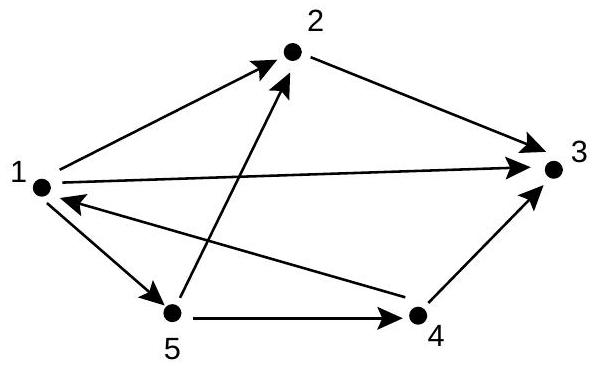
\includegraphics[max width=\textwidth, center]{2025_09_05_955b52bfc43174a24a9ag-12}

Para cada rama $(i, j)$ de $G$ denotemos por $u_{i j}$ a su capacidad y por $c_{i j}$ a su costo. Supongamos que $x$ es un flujo en $G$ que satisface $0<x_{12}<u_{12}, x_{23}=u_{23}, x_{13}=0, x_{52}=u_{52}, 0<x_{43}<u_{43}, x_{41}=u_{41}, x_{15}=0 \mathrm{y} x_{54}=0$ Entonces el grafo residual $G(x)$, donde en cada rama hemos indicado su costo, será\\
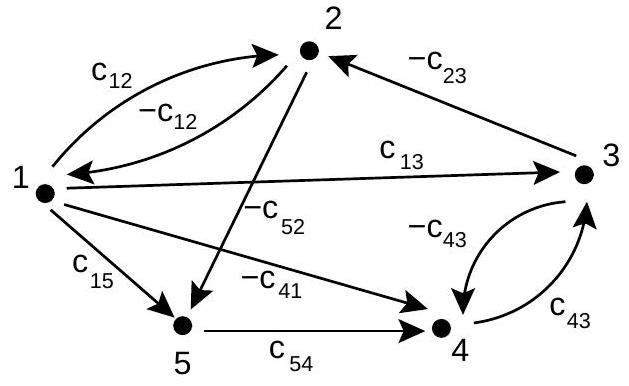
\includegraphics[max width=\textwidth, center]{2025_09_05_955b52bfc43174a24a9ag-13(3)}

De esta manera queda definida una función

$$
\psi:\{\text { circuitos aumentativos en } G\} \longrightarrow\{\text { circuitos dirigidos en } G(x)\}
$$

tal que $c(\mathcal{P})=c(\psi(\mathcal{P}))$ para todo circuito aumentativo $\mathcal{P}$ de $G$. Por razones de claridad, no definiremos formalmente esta función sino que la mostraremos en los dos siguientes ejemplos.

Ejemplo 3.3. En el grafo del ejemplo 3.2., si $\mathcal{P}$ es el circuito aumentativo indicado con trazo grueso\\
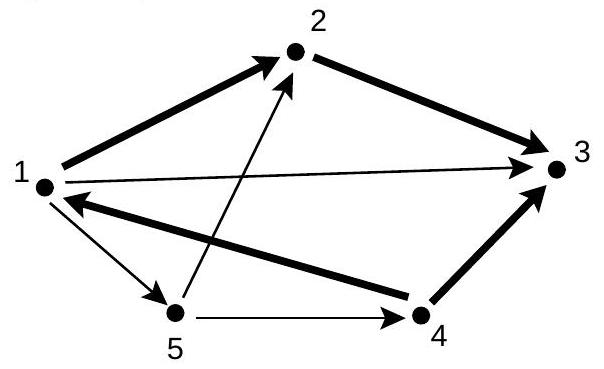
\includegraphics[max width=\textwidth, center]{2025_09_05_955b52bfc43174a24a9ag-13(2)}\\
es decir, el circuito $4 \longrightarrow 3 \longleftarrow 2 \longleftarrow 1 \longleftarrow 4$ entonces $\psi(\mathcal{P})$ es el circuito dirigido en $G(x)$\\
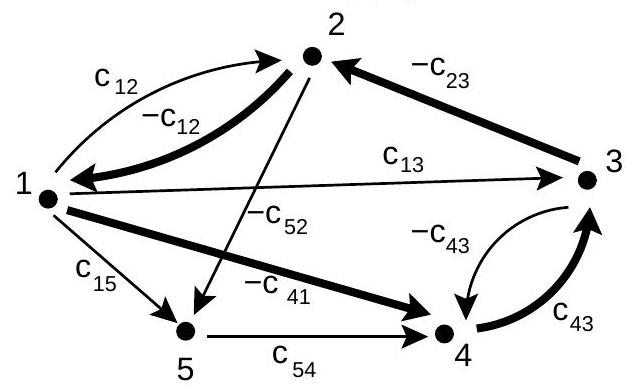
\includegraphics[max width=\textwidth, center]{2025_09_05_955b52bfc43174a24a9ag-13}

Veamos que los costos de estos circuitos coinciden: $c(\mathcal{P})=c_{43}-c_{23}-c_{12}-c_{41}=c(\psi(\mathcal{P}))$.\\
Ejemplo 3.4. Si ahora consideramos el circuito aumentativo $\mathcal{C}$ indicado con trazo grueso\\
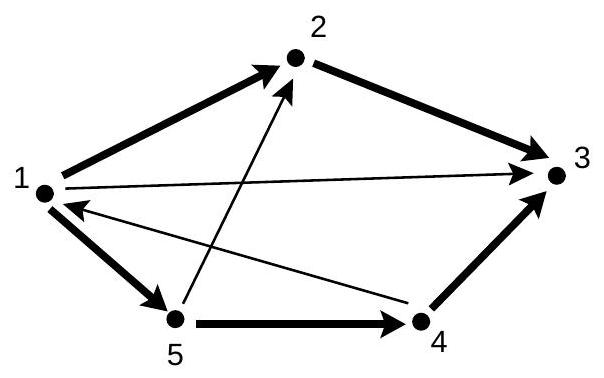
\includegraphics[max width=\textwidth, center]{2025_09_05_955b52bfc43174a24a9ag-13(1)}\\
es decir, el circuito $5 \longrightarrow 4 \longrightarrow 3 \longleftarrow 2 \longleftarrow 1 \longrightarrow 5$ entonces $\psi(\mathcal{C})$ es el circuito dirigido en $G(x)$\\
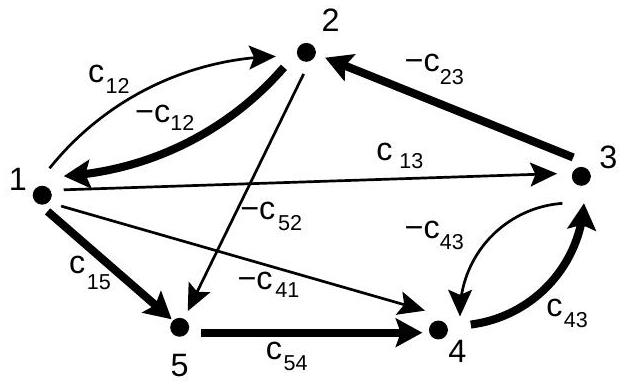
\includegraphics[max width=\textwidth, center]{2025_09_05_955b52bfc43174a24a9ag-14}

Veamos que $c(\mathcal{C})=c(\psi(\mathcal{C}))$. En efecto, $c(\mathcal{C})=c_{54}+c_{43}-c_{23}-c_{12}+c_{15}=c(\psi(\mathcal{C}))$.\\
Observación 3.5. La función $\psi$ aplica biyectivamente el conjunto de circuitos aumentativos de costo negativo en $G$ en el conjunto de circuitos dirigidos de costo negativo en $G(x)$. Por lo tanto, existe un circuito aumentativo de costo negativo en $G$ si y sólo si existe un circuito dirigido de costo negativo en $G(x)$.

Teorema 3.6. Una solución factible $x$ es óptima si y sólo si no existe un circuito aumentativo de costo negativo en $G$.\\
Demostración: $(\Longrightarrow)$ resulta de la observación 3.1.\\
$(\Longleftarrow)$ Si no existe un circuito aumentativo de costo negativo en $G$ entonces, por la observación 3.5., no existe un circuito dirigido de costo negativo en $G(x)$. Creamos un nuevo grafo $\mathcal{G}$ agregando a $G(x)$ un vértice $s$ y ramas ( $s, v$ ) para cada vértice $v$ de $G(x)$ con $\operatorname{costo} c_{s v}^{\prime}=0$. Para cada $v$, sea $y_{v}$ el costo de un camino dirigido óptimo en $\mathcal{G}$ de $s$ a $v$. Observemos que como ( $s, v$ ) es una rama de $\mathcal{G}$ entonces siempre existe al menos un camino dirigido de $s$ a $v$ y como $\mathcal{G}$ no contiene ciclos dirigidos de costo negativo entonces siempre existe un camino óptimo a $v$. Para ver que $x$ es óptimo, basta ver que ( $y_{v}$ ) satisface las condiciones i) y ii) del teorema 2.1.

Validez de i): si $x_{v w}>0$ entonces $(w, v)$ es una rama de $G(x)$ (y por lo tanto de $\mathcal{G}$ ) de costo $c_{w v}^{\prime}=-c_{v w}$. Luego, el camino dirigido óptimo de $s$ a $w$ seguido de la rama ( $w, v$ ) es un camino dirigido en $\mathcal{G}$ de $s$ a $v$ de costo $y_{w}+c_{w v}^{\prime}$ y por lo tanto debe ser $y_{v} \leq y_{w}+c_{w v}^{\prime}=y_{w}-c_{v w}$, de donde $c_{v w}+y_{v}-y_{w} \leq 0$.

Validez de ii): si $x_{v w}<u_{v w}$ entonces $(v, w)$ es una rama de $G(x)$ (y por lo tanto de $\mathcal{G}$ ) de costo $c_{v w}^{\prime}=c_{v w}$. Luego, el camino dirigido óptimo de $s$ a $v$ seguido de la rama $(v, w)$ es un camino dirigido en $\mathcal{G}$ de $s$ a $w$ de costo $y_{v}+c_{v w}^{\prime} \mathrm{y}$ por lo tanto debe ser $y_{w} \leq y_{v}+c_{v w}^{\prime}=y_{v}+c_{v w}$, de donde $c_{v w}+y_{v}-y_{w} \geq 0$ 。 $\square$

\section*{Descripción del algoritmo.}
\begin{enumerate}
  \item Encontrar una solución factible $x$. Si no existe, STOP (en tal caso el problema no tiene solución).
  \item Encontrar un circuito aumentativo $\mathcal{P}$ de costo negativo en $G$. Si no existe, STOP (en tal caso la presente solución $x$ es óptima).
  \item Calcular $\delta=\min \left\{\min \left\{u_{e}-x_{e} / e \in \mathcal{P}\right.\right.$ directa $\}, \min \left\{x_{e} / e \in \mathcal{P}\right.$ inversa $\left.\}\right\}$ y actualizar $x$ sumando $\delta$ a cada $x_{e}$ tal que $e \in \mathcal{P}$ es directa y restando $\delta$ a cada $x_{e}$ tal que $e \in \mathcal{P}$ es inversa.
\end{enumerate}

\section*{4. GOTO 2}
Observación 3.7. Para encontrar una solución factible $x$ basta resolver el problema de transshipment

$$
\begin{aligned}
& x(v, V)-x(V, v)=b_{v} \quad \forall v \in V \\
& 0 \leq x_{e} \leq u_{e} \quad \forall e \in E
\end{aligned}
$$

que estudiamos en el capítulo 3 y para encontrar un circuito aumentativo de costo negativo en $G$ basta encontrar un circuito dirigido de costo negativo en $G(x)$ (lo cual puede hacerse utilizando el algoritmo descripto en la sección 9 del capítulo 2) y luego tomar su imagen inversa por $\psi$.

\section*{4. Eliminación de la cota superior.}
El problema de hallar un flujo de mínimo costo en un grafo $G=(V, E)$

$$
\begin{aligned}
& \min \sum_{e \in E} c_{e} x_{e} \\
& x(v, V)-x(V, v)=b_{v} \quad \forall v \in V \\
& 0 \leq x_{e} \leq u_{e} \quad \forall e \in E
\end{aligned}
$$

puede escribirse en la forma

$$
\begin{aligned}
& \min c . x \\
& A x=b \\
& 0 \leq x \leq u
\end{aligned}
$$

donde $A$ es la matriz de incidencia vértice rama del grafo $G=(V, E)$.\\
Sean $\mathcal{L}=\left\{(v, w) \in E / u_{v w}=\infty\right\}, m=\# V, n=\# E$ y $k=\#(E-\mathcal{L})$. Entonces podemos eliminar la cota superior $u$ introduciendo variables de holgura, es decir reemplazando, para cada $e \in E-\mathcal{L}$, la condición $x_{e} \leq u_{e}$ por la igualdad $x_{e}+s_{e}=u_{e}$ y la condición $s_{e} \geq 0$. Luego, el problema dado es equivalente a

$$
\begin{gathered}
\min (c, 0) \cdot(x, s) \\
\left(\begin{array}{cc}
A & 0 \\
I^{\prime} & I_{k}
\end{array}\right)\binom{x}{s}=\binom{b}{u^{\prime}} \\
(x, s) \geq 0
\end{gathered}
$$

donde $I^{\prime}$ es la matriz que resulta de eliminar en la matriz identidad que tiene una fila y una columna por cada rama $e \in E$ aquellas filas correspondientes a las ramas $e \in \mathcal{L}$, el vector $u^{\prime}$ resulta de eliminar en $u$ las coordenadas $u_{e}(e \in \mathcal{L})$ y la matriz $I_{k}$ es la matriz identidad que tiene una fila y una columna por cada rama de capacidad finita, es decir, por cada rama $e \in E-\mathcal{L}$. Pero ahora la nueva matriz $\left(\begin{array}{cc}A & 0 \\ I^{\prime} & I_{k}\end{array}\right)$ no es una matriz de incidencia vértice-rama y la suma de las coordenadas del vector ( $b, u^{\prime}$ ) no tiene porqué ser nula. Veamos cómo encontrar un sistema $A^{\prime} .\binom{x}{s}=b^{\prime}$ que sea equivalente a

$$
\left(\begin{array}{cc}
A & 0 \\
I^{\prime} & I_{k}
\end{array}\right)\binom{x}{s}=\binom{b}{u^{\prime}}
$$

y donde la matriz $A^{\prime}$ sea una matriz de incidencia vértice rama y la suma de las coordenadas del vector $b^{\prime}$ sea cero.\\
La matriz $D=\left(\begin{array}{cc}A & 0 \\ I^{\prime} & I_{k}\end{array}\right)$ posee $n+k$ columnas (una para cada $e \in E$ y una para cada $e \in E-\mathcal{L}$ ) y posee $m+k$ filas (una para cada $v \in V$ y una para cada $e \in E-\mathcal{L}$ ).\\
Examinemos los coeficientes de esta matriz en cada columna. Supongamos que la columna es una de las $n$ primeras y que $e=(v, w) \in E$ es la correspondiente rama. Si $e \notin \mathcal{L}$ entonces los únicos coeficientes no nulos en esa columna son los que corresponden a las filas $v, w$ y $e=(v, w)$, que son $1,-1$ y 1 respectivamente (es decir, $d_{v e}=1, d_{w e}=-1, d_{e e}=1$ y $d_{i e}=0$ para $\left.i \neq v, w, e\right)$ y si $e \in \mathcal{L}$ entonces los únicos coeficientes no nulos en esa columna son los que corresponden a las filas $v$ y $w$, que son 1 y -1 respectivamente (es decir, $d_{v e}=1, d_{w e}=-1$ y $d_{i e}=0$ para $\left.i \neq v, w\right)$. Si, en cambio, la columna es una de las $k$ últimas, entonces corresponde a una rama $e \in E-\mathcal{L}$ y en ese caso el único coeficiente no nulo en esa columna es el que corresponde a la fila $e$ que vale 1 (es decir, $d_{e e}=1$ y $d_{i e}=0$ para $i \neq e$ ).

Haciendo en la matriz ampliada del sistema $\left(\begin{array}{cc|c}A & 0 & b \\ I^{\prime} & I_{k} & u^{\prime}\end{array}\right)$ la transformación de filas

$$
F_{u}^{\prime}=F_{u}+\sum_{\substack{e \in E-\mathcal{L} / \\ u \text { es la punta dee }}} F_{e}
$$

para cada $u \in V$ que sea la punta de una rama en $E-\mathcal{L}$ y $F_{e}^{\prime}=-F_{e}$ para cada $e \in E-\mathcal{L}$ se obtiene una matriz ( $A^{\prime} \mid b^{\prime}$ ) donde $A^{\prime}$ tiene en cada columna un 1 y un -1 y los restantes coeficientes nulos y la suma de las coordenadas de $b^{\prime}$ es igual a la suma de las coordenadas de $b$ y por lo tanto es cero. En efecto, examinemos ahora los coeficientes de $A^{\prime}$ en cada columna.

\section*{Afirmación:}
i) Si la columna es una de las $n$ primeras y que $e=(v, w) \in E$ es la correspondiente rama.\\
a) Si $e \notin \mathcal{L}$ entonces los únicos coeficientes no nulos en esa columna son los que corresponden a las filas $v$ y $e=(v, w)$, que son 1 y -1 respectivamente.\\
b) Si $e \in \mathcal{L}$ entonces los únicos coeficientes no nulos en esa columna son los que corresponden a las filas $v$ y $w$, que son 1 y -1 respectivamente.\\
ii) Si la columna es una de las $k$ últimas y $e=(v, w) \in E-\mathcal{L}$ es la correspondiente rama entonces los únicos coeficientes no nulos en esa columna son los que corresponden a las filas $w$ y $e=(v, w)$ que son 1 y -1 respectivamente.

\section*{Demostración:}
i) a) Como $d_{v e}=1, d_{w e}=-1, d_{e e}=1$ y $d_{i e}=0$ para $i \neq v, w, e$ y la transformación de filas es

$$
F_{u}^{\prime}=F_{u}+\sum_{\substack{e^{\prime} \in E-\mathcal{L} \prime \\ \text { ues la puntade } e^{\prime}}} F_{e^{\prime}}
$$

para cada $u \in V$ que sea la punta de una rama en $E-\mathcal{L}$ y $F_{e^{\prime}}^{\prime}=-F_{e^{\prime}}$ para cada $e^{\prime} \in E-\mathcal{L}$, entonces

$$
\begin{gathered}
a_{i e}^{\prime}=\left\{\begin{array}{l}
d_{i e}+\sum_{\substack{e^{\prime} \in E-\mathcal{L} / \\
i \text { esla puntade } e^{\prime}}} d_{e^{\prime} e} \quad \text { si } i \in V, i \neq w \\
d_{w e}+\sum_{\substack{e^{\prime} \in E-\mathcal{L} / \\
\text { wesla puntade } e^{\prime}}} d_{e^{\prime} e} \quad \text { si } i=w \\
-d_{i e} \quad \text { si } i \in E-\mathcal{L}
\end{array}\right. \\
= \begin{cases}d_{i e}+0 & \text { si } i \in V, i \neq w \\
d_{w e}+1 & \text { si } i=w \\
-d_{i e} & \text { si } i \in E-\mathcal{L}\end{cases} \\
= \begin{cases}1 & \text { si } i \in V, i=v \\
0 & \text { si } i \in V, i \neq v, w \\
0 & \text { si } i \in V, i=w \\
0 & \text { si } i \in E-\mathcal{L}, i \neq e \\
-1 & \text { si } i \in E-\mathcal{L}, i=e\end{cases}
\end{gathered}
$$

Dejamos como tarea al lector la demostración de i) b) y ii). $\square$\\
Ahora examinemos la columna $b^{\prime}$. Para cada $w \in V$, la fila $w$ de $b^{\prime}$ es

$$
b_{w}^{\prime}= \begin{cases}b_{w}+\sum_{v /(v, w) \in E-\mathcal{L}} u_{v w} & \text { si } w \text { es la punta de alguna rama en } E-\mathcal{L} \\ b_{w} & \text { si no }\end{cases}
$$

y para cada $e=(v, w) \in E-\mathcal{L}$ la coordenada $e$ de $b^{\prime}$ es $-u_{v w}$ Luego,

$$
\begin{aligned}
& \sum_{w} b_{w}^{\prime}+\sum_{(v, w) \in E-\mathcal{L}} b_{v w}^{\prime}= \\
= & \sum_{w} b_{w}+\sum_{w} \sum_{v /(v, w) \in E-\mathcal{L}} u_{v w}+\sum_{(v, w) \in E-\mathcal{L}}-u_{v w}= \\
= & \sum_{w} b_{w}+\sum_{(v, w) \in E-\mathcal{L}} u_{v w}+\sum_{(v, w) \in E-\mathcal{L}}-u_{v w}= \\
= & \sum_{w} b_{w}=0
\end{aligned}
$$

Luego, el problema de hallar un flujo de mínimo costo en $G$ es equivalente a

$$
\begin{gathered}
\min (c, 0) \cdot(x, s) \\
A^{\prime}\binom{x}{s}=b^{\prime} \\
(x, s) \geq 0
\end{gathered}
$$

donde $A^{\prime}$ es una matriz de incidencia vértice-rama y la suma de las coordenadas de $b^{\prime}$ es cero.\\
Si consideramos el grafo $G^{\prime}$ que se obtiene de $G$ agregando un vértice $e$ por cada rama de capacidad finita $e$ de $G$ y reemplazando en $G$ cada rama de capacidad finita $e=(v, w)$ por dos ramas, una rama ( $v, e$ ) y otra rama ( $w, e$ ) resulta que, ordenando convenientemente los vértices y las ramas de $G^{\prime}$, la matriz de incidencia vértice-rama de $G^{\prime}$ es la matriz $A^{\prime}$.\\
Si a cada rama $e$ de $G^{\prime}$ tal que $e$ era una rama de $G$ de capacidad infinita le asignamos costo $c_{e}$, capacidad infinita y denotamos por $x_{e}$ su flujo, a cada rama $(v, e)$ de $G^{\prime}$ tal que $v$ es la cola de $e$ le asignamos costo $c_{e}$, capacidad infinita y denotamos por $x_{e}$ su flujo y a cada rama ( $v, e$ ) de $G^{\prime}$ tal que $v$ es la punta de $e$ le asignamos costo cero, capacidad infinita y denotamos por $s_{e}$ a su flujo entonces tomando al vector $b^{\prime}$ como vector de oferta-demanda de los vértices de $G^{\prime}$ (que tiene una coordenada por cada vértice de $G$ y por cada rama de $G$ de capacidad finita, es decir, una coordenada por cada vértice de $G^{\prime}$ ), el problema resulta ser el problema de hallar un flujo de mínimo costo en $G^{\prime}$. Si ( $x, s$ ) es un flujo de mínimo costo en $G^{\prime}$ entonces $x$ es un flujo de mínimo costo en $G$.\\
Observación 4.1. El grafo $G$ es conexo si y sólo si el grafo $G^{\prime}$ lo es.\\
Ejemplo 4.2 Consideremos el grafo\\
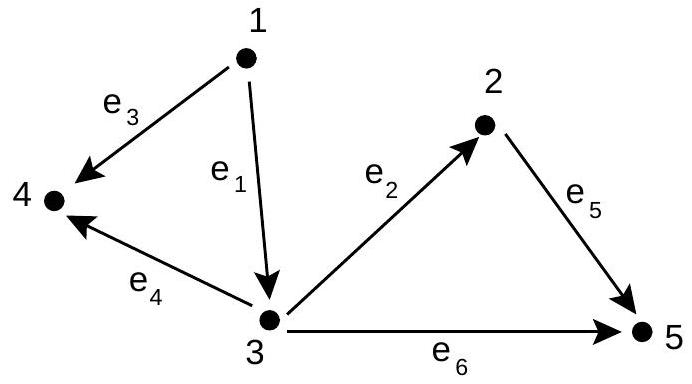
\includegraphics[max width=\textwidth, center]{2025_09_05_955b52bfc43174a24a9ag-17}\\
cuya matriz de incidencia vértice-rama es

$$
A=\left(\begin{array}{cccccc}
1 & 0 & 1 & 0 & 0 & 0 \\
0 & -1 & 0 & 0 & 1 & 0 \\
-1 & 1 & 0 & 1 & 0 & 1 \\
0 & 0 & -1 & -1 & 0 & 0 \\
0 & 0 & 0 & 0 & -1 & -1
\end{array}\right)
$$

y supongamos que $e_{1}, e_{3}, e_{5}$ y $e_{6}$ son las ramas de capacidad finita, es decir, $\mathcal{L}=\left\{e_{2}, e_{4}\right\}$.\\
Entonces, agregando una variable de holgura para cada rama $e \notin \mathcal{L}$, el problema puede plantearse en la forma

$$
\begin{gathered}
\min \sum_{i=1}^{6} c_{e_{i}} x_{e_{i}}+0 . s_{e_{1}}+0 . s_{e_{3}}+0 . s_{e_{5}}+0 . s_{e_{6}} \\
\left(\begin{array}{cccccc}
1 & 0 & 1 & 0 & 0 & 0 \\
0 & -1 & 0 & 0 & 1 & 0 \\
-1 & 1 & 0 & 1 & 0 & 1 \\
0 & 0 & -1 & -1 & 0 & 0 \\
0 & 0 & 0 & 0 & -1 & -1
\end{array}\right) \cdot\left(\begin{array}{l}
x_{e_{1}} \\
x_{e_{2}} \\
x_{e_{3}} \\
x_{e_{4}} \\
x_{e_{5}} \\
x_{e_{6}}
\end{array}\right)=\left(\begin{array}{l}
b_{1} \\
b_{2} \\
b_{3} \\
b_{4} \\
b_{5}
\end{array}\right) \\
x_{e_{1}}+s_{e_{1}}=u_{e_{1}} \\
x_{e_{3}}+s_{e_{3}}=u_{e_{3}} \\
x_{e_{5}}+s_{e_{5}}=u_{e_{5}} \\
x_{e_{6}}+s_{e_{6}}=u_{e_{6}} \\
x_{e} \geq 0(e \in E) \mathrm{y} s_{e} \geq 0(e \in E-\mathcal{L})
\end{gathered}
$$

lo que puede escribirse

$$
\begin{gathered}
\min \sum_{i=1}^{6} c_{e_{i}} x_{e_{i}}+0 . s_{e_{1}}+0 . s_{e_{3}}+0 . s_{e_{5}}+0 . s_{e_{6}} \\
\left(\begin{array}{cccccccccc}
1 & 0 & 1 & 0 & 0 & 0 & 0 & 0 & 0 & 0 \\
0 & -1 & 0 & 0 & 1 & 0 & 0 & 0 & 0 & 0 \\
-1 & 1 & 0 & 1 & 0 & 1 & 0 & 0 & 0 & 0 \\
0 & 0 & -1 & -1 & 0 & 0 & 0 & 0 & 0 & 0 \\
0 & 0 & 0 & 0 & -1 & -1 & 0 & 0 & 0 & 0 \\
1 & 0 & 0 & 0 & 0 & 0 & 1 & 0 & 0 & 0 \\
0 & 0 & 1 & 0 & 0 & 0 & 0 & 1 & 0 & 0 \\
0 & 0 & 0 & 0 & 1 & 0 & 0 & 0 & 1 & 0 \\
0 & 0 & 0 & 0 & 0 & 1 & 0 & 0 & 0 & 1
\end{array}\right) \cdot\left(\begin{array}{l}
x_{e_{1}} \\
x_{e_{2}} \\
x_{e_{3}} \\
x_{e_{4}} \\
x_{e_{5}} \\
x_{e_{6}} \\
s_{e_{1}} \\
s_{e_{3}} \\
s_{e_{5}} \\
s_{e_{6}}
\end{array}\right)=\left(\begin{array}{c}
b_{1} \\
b_{2} \\
b_{3} \\
b_{4} \\
b_{5} \\
u_{e_{1}} \\
u_{e_{3}} \\
u_{e_{5}} \\
u_{e_{6}}
\end{array}\right) \\
x_{e} \geq 0(e \in E) \mathrm{y} s_{e} \geq 0(e \in E-\mathcal{L})
\end{gathered}
$$

Haciendo la transformación de filas

$$
F_{u}^{\prime}=F_{u}+\sum_{\substack{e \in E-\mathcal{L} / \\ \text { u eslapunta dee }}} F_{e}
$$

para cada $u \in V$ que sea la punta de una rama en $E-\mathcal{L}$ y

$$
F_{e}^{\prime}=-F_{e}
$$

para cada $e \in E-\mathcal{L}$ en la matriz ampliada del sistema

$$
\left(\begin{array}{cccccccccc:c}
1 & 0 & 1 & 0 & 0 & 0 & 0 & 0 & 0 & 0 & b_{1} \\
0 & -1 & 0 & 0 & 1 & 0 & 0 & 0 & 0 & 0 & b_{2} \\
-1 & 1 & 0 & 1 & 0 & 1 & 0 & 0 & 0 & 0 & b_{3} \\
0 & 0 & -1 & -1 & 0 & 0 & 0 & 0 & 0 & 0 & b_{4} \\
0 & 0 & 0 & 0 & -1 & -1 & 0 & 0 & 0 & 0 & b_{5} \\
1 & 0 & 0 & 0 & 0 & 0 & 1 & 0 & 0 & 0 & u_{e_{1}} \\
0 & 0 & 1 & 0 & 0 & 0 & 0 & 1 & 0 & 0 & u_{e_{3}} \\
0 & 0 & 0 & 0 & 1 & 0 & 0 & 0 & 1 & 0 & u_{e_{5}} \\
0 & 0 & 0 & 0 & 0 & 1 & 0 & 0 & 0 & 1 & u_{e_{6}}
\end{array}\right)
$$

se obtiene la matriz

$$
\left(A^{\prime} \mid b^{\prime}\right)=\left(\begin{array}{cccccccccc:c}
1 & 0 & 1 & 0 & 0 & 0 & 0 & 0 & 0 & 0 & b_{1} \\
0 & -1 & 0 & 0 & 1 & 0 & 0 & 0 & 0 & 0 & b_{2} \\
0 & 1 & 0 & 1 & 0 & 1 & 1 & 0 & 0 & 0 & b_{3}+u_{e_{1}} \\
0 & 0 & 0 & -1 & 0 & 0 & 0 & 1 & 0 & 0 & b_{4}+u_{e_{3}} \\
0 & 0 & 0 & 0 & 0 & 0 & 0 & 0 & 1 & 1 & b_{5}+u_{e_{5}}+u_{e_{6}} \\
-1 & 0 & 0 & 0 & 0 & 0 & -1 & 0 & 0 & 0 & -u_{e_{1}} \\
0 & 0 & -1 & 0 & 0 & 0 & 0 & -1 & 0 & 0 & -u_{e_{3}} \\
0 & 0 & 0 & 0 & -1 & 0 & 0 & 0 & -1 & 0 & -u_{e_{5}} \\
0 & 0 & 0 & 0 & 0 & -1 & 0 & 0 & 0 & -1 & -u_{e_{6}}
\end{array}\right)
$$

Luego el problema dado para el grafo $G$ resulta equivalente a

$$
\begin{gathered}
\min \sum_{i=1}^{6} c_{e_{i}} x_{e_{i}}+0 . s_{e_{1}}+0 . s_{e_{3}}+0 . s_{e_{5}}+0 . s_{e_{6}} \\
\left(\begin{array}{cccccccccc}
1 & 0 & 1 & 0 & 0 & 0 & 0 & 0 & 0 & 0 \\
0 & -1 & 0 & 0 & 1 & 0 & 0 & 0 & 0 & 0 \\
0 & 1 & 0 & 1 & 0 & 1 & 1 & 0 & 0 & 0 \\
0 & 0 & 0 & -1 & 0 & 0 & 0 & 1 & 0 & 0 \\
0 & 0 & 0 & 0 & 0 & 0 & 0 & 0 & 1 & 1 \\
-1 & 0 & 0 & 0 & 0 & 0 & -1 & 0 & 0 & 0 \\
0 & 0 & -1 & 0 & 0 & 0 & 0 & -1 & 0 & 0 \\
0 & 0 & 0 & 0 & -1 & 0 & 0 & 0 & -1 & 0 \\
0 & 0 & 0 & 0 & 0 & -1 & 0 & 0 & 0 & -1
\end{array}\right) \cdot\left(\begin{array}{c}
x_{e_{1}} \\
x_{e_{2}} \\
x_{e_{3}} \\
x_{e_{4}} \\
x_{e_{5}} \\
x_{e_{6}} \\
s_{e_{1}} \\
s_{e_{3}} \\
s_{e_{5}} \\
s_{e_{6}}
\end{array}\right)=\left(\begin{array}{c}
b_{1} \\
b_{2} \\
b_{3}+u_{e_{1}} \\
b_{4}+u_{e_{3}} \\
b_{5}+u_{e_{5}}+u_{e_{6}} \\
-u_{e_{1}} \\
-u_{e_{3}} \\
-u_{e_{5}} \\
-u_{e_{6}}
\end{array}\right) \\
s_{e} \geq 0 \\
(e \in E)
\end{gathered}
$$

que puede pensarse como un problema de flujo de mínimo costo en el grafo $G^{\prime}$, donde ninguna rama tiene restricciones de capacidad\\
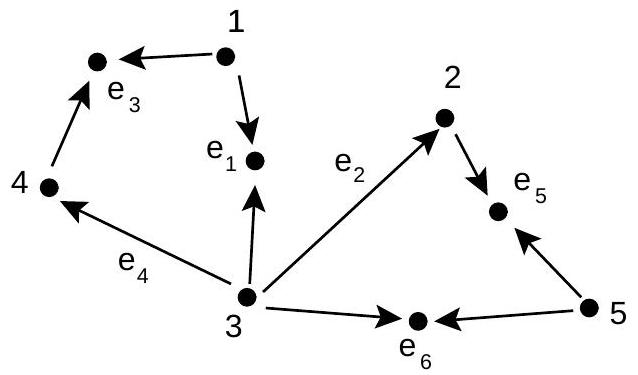
\includegraphics[max width=\textwidth, center]{2025_09_05_955b52bfc43174a24a9ag-19}\\
y donde el vector de oferta-demanda de los vértices de $G^{\prime}$ es el vector

$$
b^{\prime}=\left(b_{1}, b_{2}, b_{3}+u_{e_{1}}, b_{4}+u_{e_{3}}, b_{5}+u_{e_{5}}+u_{e_{6}},-u_{e_{1}},-u_{e_{3}},-u_{e_{5}},-u_{e_{6}}\right)
$$

En efecto, basta tomar para los vértices de $G^{\prime}$ el orden $1,2,3,4,5, e_{1}, e_{3}, e_{5}, e_{6}$ y para las ramas el orden $\left(1, e_{1}\right), e_{2},\left(1, e_{3}\right), e_{4},\left(2, e_{5}\right),\left(3, e_{6}\right),\left(3, e_{1}\right),\left(4, e_{3}\right),\left(5, e_{5}\right),\left(5, e_{6}\right)$ (con lo cual $A^{\prime}$ resulta la matriz de incidencia vértice rama de $G^{\prime}$ ) y llamar $x_{e_{1}}$ al flujo de la rama ( $1, e_{1}$ ), $x_{e_{2}}$ al flujo de la rama $e_{2}, x_{e_{3}}$ al flujo de la rama $\left(1, e_{3}\right), x_{e_{4}}$ al flujo de la rama $e_{4}, x_{e_{5}}$ al flujo de la rama $\left(2, e_{5}\right), x_{e_{6}}$ al flujo de la rama $\left(3, e_{6}\right), s_{e_{1}}$ al flujo de la rama $\left(3, e_{1}\right), s_{e_{3}}$ al flujo de la rama $\left(4, e_{3}\right), s_{e_{5}}$ al flujo de la rama $\left(5, e_{5}\right)$ y $s_{e_{6}}$ al flujo de la rama $\left(5, e_{6}\right)$. En este caso el grafo $G$ es conexo y por lo tanto el grafo $G^{\prime}$ también lo es.

\section*{5. El método "simplex" para un grafo conexo.}
Veremos ahora otro algoritmo para resolver el problema del flujo de mínimo costo que puede aplicarse en el caso en que el grafo $G$ es conexo. Este algoritmo es similar al algoritmo simplex que vimos en el capítulo 1. El papel que antes jugaban las soluciones básicas factibles lo jugarán ahora las tree solutions (ver definición 5.1. más abajo) y el que jugaba el correspondiente vector ( $i_{1}, \ldots, i_{m}$ ) lo jugará un spanning tree de $G$. Notemos que cuando $E$ es conexo entonces existe algún spanning tree de $G$ (ver capítulo 2 ).\\
Por lo visto en la sección anterior y teniendo en cuenta la observación 4.1., podemos suponer que las ramas no tienen restricciones de capacidad.

Sea $G=(V, E)$ un grafo dirigido y conexo donde cada vértice $v$ tiene asignado un número real $b_{v}$ y cada rama $e \in E$ tiene asignado un costo $c_{e}$. Supondremos que $\sum_{v} b_{v}=0$. Describiremos un algoritmo que resuelve el problema de programación lineal en forma standard


\begin{align*}
& \min c . x \\
& x(v, V)-x(V, v)=b_{v} \quad \forall v \in V  \tag{2}\\
& x_{e} \geq 0 \quad \forall e \in E
\end{align*}


Definición 5.1. Diremos que $x$ es una tree solution si es una solución factible de (2) y existe un spanning tree $T$ de $G$ tal que $x_{e}=0$ para todo $e \in E / e \notin T$.

Como dijimos antes, las tree solutions jugarán un papel similar al de las soluciones básicas factibles (ver definiciones 3.5. y 3.12., capítulo 1). Notemos que si $x$ es una tree solution y $T$ es un spanning tree tal que $x_{e}=0$ para $e \notin T$, podría ocurrir que $x_{e}=0$ para algún $e \in T$. En este caso diremos que $x$ es una tree solution degenerada. Las tree solutions degeneradas son el análogo a las soluciones básicas factibles degeneradas (ver definición 3.9 del capítulo 1).

El siguiente resultado es el análogo al teorema fundamental de la programación lineal (ver teorema 3.13, capítulo 1).

Teorema 5.2. Se verifican\\
i) Si (2) tiene una solución factible entonces tiene una tree solution.\\
ii) Si (2) tiene una solución óptima entonces tiene una tree solution que es óptima.

Demostración: i) Sea $x$ una solución factible de (2).\\
Si $x$ no es una tree solution entonces $E^{\prime}=\left\{e \in E / x_{e}>0\right\}$ contiene por lo menos un ciclo. En efecto, si $x$ no es una tree solution y $E^{\prime}$ no contiene ciclos, entonce ( $V, E^{\prime}$ ) es acíclico pero no puede ser un spanning tree de $G$. Luego debe ser disconexo. Entonces podemos agregarle ramas de manera que siga siendo acíclico hasta obtener un spanning tree $T$ de $G$. Observando que $x_{e}=0$ para cada una de las ramas $e$ que no pertenecen a $T$ (ya que toda rama de $E^{\prime}$ es una rama de $T$ ) resulta que $T$ es un spanning tree de $G$ que satisface $x_{e}=0 \forall e \notin T$. Pero esto no puede ocurrir ya que $x$ no era una tree solution. Luego $E^{\prime}$ contiene al menos un ciclo C.

Sea $\delta=\min \left\{x_{e} / e \in \mathcal{C}\right\}$ y sea $e_{0}$ tal que $x_{e_{0}}=\delta$. Luego $\delta>0 \mathrm{y}$, como no hay restricciones de capacidad, restando $\delta$ al flujo de las ramas de $\mathcal{C}$ que tienen la misma dirección que $e_{0}$ y sumando $\delta$ al flujo de las ramas de $\mathcal{C}$ que tienen dirección contraria a $e_{0}$ obtenemos una nueva solución factible $x^{\prime}$ que satisface $x_{e_{0}}^{\prime}=0$. Además, como $x_{e}^{\prime}=x_{e}$ para toda rama $e \notin \mathcal{C}$ y $\mathcal{C}$ está contenido en $E^{\prime}$ entonces $x_{e}^{\prime}=0 \forall e \notin E^{\prime}$. Luego $\left\{e \in E / x_{e}^{\prime}>0\right\}$ es un subconjunto de $E^{\prime}$ y por lo tanto todo ciclo contenido en él es un ciclo contenido en $E^{\prime}$. Como además $e_{0} \notin\left\{e \in E / x_{e}^{\prime}>0\right\}$ entonces $\mathcal{C}$ no es un ciclo contenido en $\left\{e \in E / x_{e}^{\prime}>0\right\}$.\\
En resumen, a partir de $x$ hemos construído una solución factible $x^{\prime}$ tal que $\left\{e \in E / x_{e}^{\prime}>0\right\}$ contiene por lo menos un ciclo menos que $\left\{e \in E / x_{e}>0\right\}$. Iterando este procedimiento, en un número finito de pasos\\
obtendremos una solución factible $\bar{x}$ tal que $\left\{e \in E / \bar{x}_{e}>0\right\}$ no contenga ciclos y por lo tanto $\bar{x}$ será una tree solution.\\
ii) Ahora supongamos que $x$ es una solución óptima de (2).

Si $x$ no es una tree solution entonces $\left\{e \in E / x_{e}>0\right\}$ contiene un ciclo $\mathcal{C}$. Como $x$ es óptimo el costo de $\mathcal{C}$ debe ser cero. En efecto, si $\mathcal{C}$ tuviese costo no nulo entonces, al no haber restricciones de capacidad, recorriendo $\mathcal{C}$ en alguna de las dos direcciones tendríamos un circuito aumentativo de costo negativo, lo que contradice la optimalidad de $x$ (ver observación 3.1.). Luego, procediendo como en i) podemos encontrar una solución factible $x^{\prime}$ tal que $\left\{e \in E / x_{e}^{\prime}>0\right\}$ contiene por lo menos un ciclo menos que $\left\{e \in E / x_{e}>0\right\}$ y como $c(\mathcal{C})=0$ entonces $c x=c x^{\prime}$, es decir, $x^{\prime}$ es también una solución óptima de (2). Iterando este procedimiento un número finito de veces obtendremos una tree solution óptima\\
Fijemos un vértice $s$ en $G$ al que llamaremos raíz. Dado un spanning tree $T$ de $G$, si $h$ es una rama de $T$ denotaremos por $R(T, h)$ al conjunto formado por la raíz $s$ y todos aquellos vértices $v$ de $G$ distintos de $s$ tales que el único camino en $T$ de $s$ a $v$ no contiene a la rama $h$. Notemos que $s \in R(T, h)$.

Lema 5.3. Si $v$ y $w$ son vértices de $G$ y $h=(p, q)$ es una rama de $T$ entonces

$$
\{(v, w) \in T / v \in R(T, h), w \notin R(T, h)\}= \begin{cases}\{h\} & \text { si } p \in R(T, h) \\ \emptyset & \text { si } p \notin R(T, h)\end{cases}
$$

y

$$
\{(w, v) \in T / v \in R(T, h), w \notin R(T, h)\}= \begin{cases}\{h\} & \text { si } p \notin R(T, h) \\ \emptyset & \text { si } p \in R(T, h)\end{cases}
$$

Demostración: Probemos la primera iguladad. Si $v \in R(T, h), w \notin R(T, h)$ y $(v, w) \in T$, entonces el único camino en $T$ de $s$ a $v$ no contiene a $h$ y el único camino en $T$ de $s$ a $w$ sí. Luego, el único camino en $T$ de $s$ a $v$ no puede pasar por $w$ y como $(v, w) \in T$ agregándole la rama $(v, w)$ se obtiene un camino en $T$ de $s$ a $w$. Por unicidad, ese debe ser el único camino en $T$ de $s$ a $w$ y como ese camino contiene a $h$ y el camino de $s$ a $v$ no, entonces debe ser $h=(v, w)$.\\
Luego, $\{(v, w) \in T / v \in R(T, h), w \notin R(T, h)\} \subseteq\{h\}$ y vale la otra inclusión si y sólo si $p \in R(T, h)$ y $q \notin R(T, h)$.\\
Luego el resultado se sigue observando que

$$
p \in R(T, h) \text { y } q \notin R(T, h) \Longleftrightarrow p \in R(T, h)
$$

En efecto, si $p \in R(T, h)$ entonces el único camino en $T$ de $s$ a $p$ no contiene a $h$. Luego, agregando a ese camino la rama $h \in T$ se obtiene el único camino en $T$ de $s$ a $q$. Luego el camino en $T$ de $s$ a $q$ contiene a $h$ y por lo tanto $q \notin R(T, h)$.\\
La segunda igualdad, que dejamos a cargo del lector, se prueba de manera análoga. ㅁ\\
Proposición 5.4. Sea $x$ una tree solution y sea $T$ un spanning tree de $G$ tal que $x_{e}=0 \forall e \notin T$. Entonces $x$ queda determinada por $T$.\\
Demostración: Como $x_{e}=0 \forall e \notin T$, para conocer $x$ basta conocer $x_{h}$ para cada $h \in T$. Sea $h=(p, q) \in T$. Entonces

$$
x_{h}= \begin{cases}\sum_{v \in R(T, h)} b_{v} & \text { si } p \in R(T, h) \\ -\sum_{v \in R(T, h)} b_{v} & \text { si } p \notin R(T, h)\end{cases}
$$

En efecto, como $x_{e}=0$ para $e \notin T$

$$
\begin{aligned}
b_{v} & =\sum_{w /(v, w) \in E} x_{v w}-\sum_{w /(w, v) \in E} x_{w v}= \\
& =\sum_{w /(v, w) \in T} x_{v w}-\sum_{w /(w, v) \in T} x_{w v}
\end{aligned}
$$

Luego,

$$
\begin{aligned}
\sum_{v \in R(T, h)} b_{v} & =\sum_{v \in R(T, h)}\left(\sum_{w /(v, w) \in T} x_{v w}-\sum_{w /(w, v) \in T} x_{w v}\right)= \\
& =\sum_{v \in R(T, h)} \sum_{\substack{w \in R(T, h) / \\
(v, w) \in T}} x_{v w}+\sum_{v \in R(T, h)} \sum_{\substack{w \notin R(T, h) / \\
(v, w) \in T}} x_{v w}- \\
& -\sum_{v \in R(T, h)} \sum_{\substack{w \in R(T, h) / \\
(w, v) \in T}} x_{w v}-\sum_{v \in R(T, h)} \sum_{\substack{w \notin R(T, h) / \\
(w, v) \in T}} x_{w v}= \\
& =\sum_{v \in R(T, h)} \sum_{\substack{w \notin R(T, h) / \\
(v, w) \in T}} x_{v w}-\sum_{v \in R(T, h)} \sum_{\substack{w \notin R(T, h) / \\
(w, v) \in T}} x_{w v}= \\
& =\sum_{v \in R(T, h), w \notin R(T, h) /} x_{v w}-\sum_{v \in R(T, h), w \notin R(T, h) /} x_{w v}
\end{aligned}
$$

Ahora, usando el lema 5.3. se tiene que

$$
\sum_{v \in R(T, h)} b_{v}=\sum_{\substack{v \in R(T, h), w \notin R(T, h) / \\(v, w) \in T}} x_{v w}-\sum_{\substack{v \in R(T, h), w \notin R(T, h) / \\(w, v) \in T}} x_{w v}= \begin{cases}x_{h} & \text { si } p \in R(T, h) \\ -x_{h} & \text { si } p \notin R(T, h)\end{cases}
$$

como queríamos probar.\\
Corolario 5.5 Existen finitas tree solutions de $G$.\\
Sea $x$ una tree solution y sea $T$ un spanning tree de $G$ tal que $x_{e}=0$ para todo $e \notin T$. Para cada $v \in V$, $v \neq s$, denotemos por $y_{v}$ al costo del único camino en $T$ de $s$ a $v$, y sea $y_{s}=0$.

Observación 5.6. Dados dos vértices $v$ y $w$ de $G$, si $\mathcal{P}$ es el único camino en $T$ de $v$ a $w$ entonces el único camino en $T$ de $w$ a $v$ es el que resulta de recorrer $\mathcal{P}$ en sentido contrario. Denotaremos por $-\mathcal{P}$ a este camino. Luego, las ramas de $\mathcal{P}$ que son directas son las ramas de $-\mathcal{P}$ que son inversas y las ramas de $\mathcal{P}$ que son inversas son las ramas de $-\mathcal{P}$ que son directas, de donde se tiene que $c(-\mathcal{P})=-c(\mathcal{P})$. Por ejemplo, si $T$ es\\
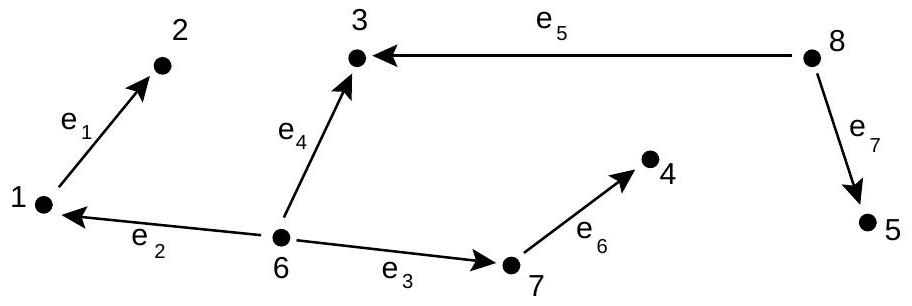
\includegraphics[max width=\textwidth, center]{2025_09_05_955b52bfc43174a24a9ag-22(1)}\\
el único camino $\mathcal{P}$ de 2 a 5 es $\left(e_{1}, e_{2}, e_{4}, e_{5}, e_{7}\right)$. En este camino las ramas $e_{4}$ y $e_{7}$ son directas y las ramas $e_{1}, e_{2}$ y $e_{5}$ son inversas. Luego, el único camino $-\mathcal{P}$ en $T$ de 5 a 2 es el camino ( $e_{7}, e_{5}, e_{4}, e_{2}, e_{1}$ ) cuyas ramas directas son $e_{1}, e_{2}$ y $e_{5}$ y cuyas ramas inversas son $e_{4}$ y $e_{7}$.

Observación 5.7. Si $v$ y $w$ son dos vértices de $G$ entonces el costo del único camino $\mathcal{P}$ en $T$ de $v$ a $w$ es $y_{w}-y_{v}$. En efecto, esto es claro si $v=s$ o $w=s$ ya que $y_{s}=0$ por definición. Supongamos entonces que $v, w \neq s$ y sea $\mathcal{C}$ el único camino en $T$ de $s$ a $v$. Entonces $y_{v}=c(\mathcal{C})$.\\
Si la situación es\\
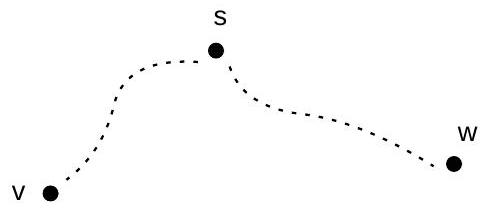
\includegraphics[max width=\textwidth, center]{2025_09_05_955b52bfc43174a24a9ag-22}\\
entonces $\mathcal{P}$ es igual a $-\mathcal{C}$ seguido del único camino de $s$ a $w$. En este caso $c(\mathcal{P})=-y_{v}+y_{w}$. Si en cambio tenemos la situación\\
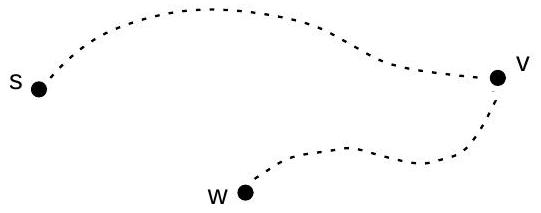
\includegraphics[max width=\textwidth, center]{2025_09_05_955b52bfc43174a24a9ag-23}\\
entonces el único camino de $s$ a $w$ es $\mathcal{C}$ seguido de $\mathcal{P}$. Luego, $y_{w}=c(\mathcal{C})+c(\mathcal{P})=y_{v}+c(\mathcal{P})$ y por lo tanto $c(\mathcal{P})=y_{w}-y_{v}$. Por último, si la situación es\\
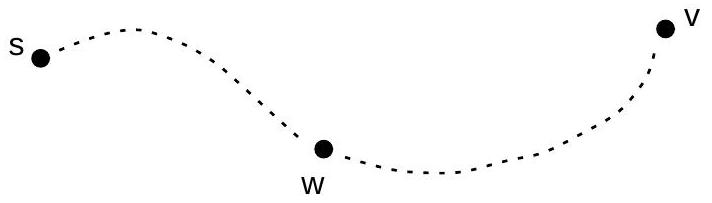
\includegraphics[max width=\textwidth, center]{2025_09_05_955b52bfc43174a24a9ag-23(2)}\\
entonces el único camino de $s$ a $w$ seguido de $-\mathcal{P}$ es un camino de $s$ a $v$ y por lo tanto debe ser el camino $\mathcal{C}$. Luego debe ser $y_{w}+c(-\mathcal{P})=c(\mathcal{C})=y_{v}$, es decir, $y_{w}-c(\mathcal{P})=y_{v}$ y por lo tanto también en este caso $c(\mathcal{P})=y_{w}-y_{v}$.\\
Recordemos que si $\left(y_{v}\right)_{v \in V}$ verifica las condiciones del teorema 2.1 entonces $x$ es una solución óptima del problema. Como en este caso no hay restricciones de capacidad, es decir, $u_{e}=\infty$ para todo $e \in E$, entonces $x_{e}<u_{e} \forall e \in E$. Luego las condiciones resultan ser\\
i) $x_{v w}>0 \Longrightarrow c_{v w}+y_{v}-y_{w} \leq 0$\\
ii) $c_{v w}+y_{v}-y_{w} \geq 0$ para todo $(v, w) \in E$

Proposición 5.8. Si $\left(y_{v}\right)_{v \in V}$ verifica\\
i') $c_{v w}+y_{v}-y_{w}=0$ para todo $(v, w) \in T$\\
ii') $c_{v w}+y_{v}-y_{w} \geq 0$ para todo $(v, w) \notin T$\\
entonces $x$ es óptimo.\\
Demostración: Veamos que i') y ii') implican i) y ii). Como $x_{e}=0 \forall e \notin T$, si $x_{v w}>0$ entonces $(v, w) \in T$. Luego, por i') $c_{v w}+y_{v}-y_{w}=0 \mathrm{y}$ por lo tanto vale i).\\
Veamos ahora que vale ii). Dado $(v, w) \in E$, si $(v, w) \in T$ entonces $c_{v w}+y_{v}-y_{w}=0$ y si $(v, w) \notin T$ entonces $c_{v w}+y_{v}-y_{w} \geq 0$. 口\\
Corolario 5.9. Para todo $(v, w) \in T$ se verifica que $c_{v w}+y_{v}-y_{w}=0$. Por lo tanto, si $\left(y_{v}\right)_{v \in V}$ verifica $c_{v w}+y_{v}-y_{w} \geq 0$ para todo $(v, w) \notin T$ entonces $x$ es óptimo.\\
Demostración: Sea $(v, w) \in T$. Por la observación 5.7. el costo del único camino en $T$ de $v$ a $w$ es $y_{w}-y_{v}$. Pero como $(v, w) \in T$ este camino debe ser $(v, w)$ cuyo costo es $c_{v w}$. Luego $c_{v w}=y_{w}-y_{v}=0$ de donde $c_{v w}+y_{v}-y_{w}=0$. Luego, por la proposición 5.8., si $\left(y_{v}\right)_{v \in V}$ verifica $c_{v w}+y_{v}-y_{w} \geq 0$ para todo $(v, w) \notin T$ resulta que $x$ es óptimo.\\
Supongamos que para alguna rama $(v, w) \notin T$ sea $c_{v w}+y_{v}-y_{w}<0$. Entonces el grafo obtenido agregando a $T$ la rama ( $v, w$ ) contiene un único ciclo $\mathcal{C}$.\\
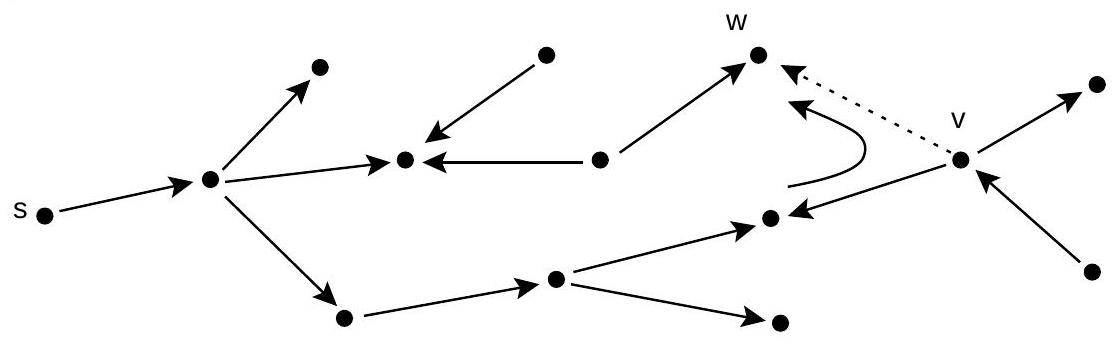
\includegraphics[max width=\textwidth, center]{2025_09_05_955b52bfc43174a24a9ag-23(1)}

Si recorremos este ciclo en el sentido de $(v, w)$ se tiene que su costo es $c_{v w}$ más el costo del único camino en $T$ de $w$ a $v$, es decir, $c(\mathcal{C})=c_{v w}+y_{v}-y_{w}$ (ver observación 5.7.) y por lo tanto $c(\mathcal{C})<0$.\\
Supongamos que existe al menos una rama inversa en $\mathcal{C}$. Sea $\delta=\min \left\{x_{e} / e \in \mathcal{C}\right.$ es inversa $\}$. Entonces $\delta \geq 0$ y sumando $\delta$ al flujo de las ramas directas y restando $\delta$ al flujo de las ramas inversas obtenemos un nuevo flujo factible $x^{\prime}$.\\
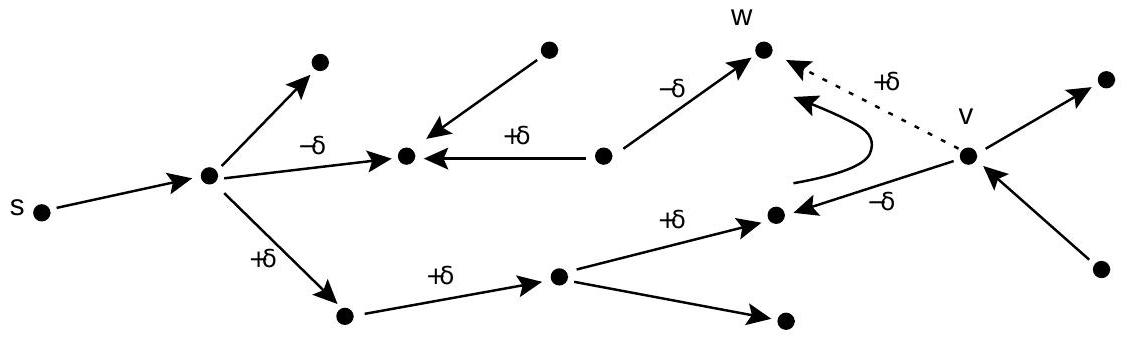
\includegraphics[max width=\textwidth, center]{2025_09_05_955b52bfc43174a24a9ag-24}

Si $e_{0} \in \mathcal{C}$ es la rama inversa tal que $\delta=x_{e_{0}}$ entonces $x_{e_{0}}^{\prime}=x_{e_{0}}-\delta=0$. Si ahora consideramos el spanning tree $T^{\prime}$ que resulta de quitarle a $T$ la rama $e_{0}$ y agregarle la rama $(v, w)$ entonces $x_{e}^{\prime}=0$ para todo $e \notin T^{\prime}$ (luego, $x^{\prime}$ es una tree solution) y, por la observación 3.1. se tiene que

$$
c x^{\prime}=c x+\delta . c(\mathcal{C}) \leq c x
$$

Observemos que para cada $u \neq s$ el costo $y_{u}^{\prime}$ del único camino en $T^{\prime}$ de $s$ a $u$ es

$$
y_{u}^{\prime}= \begin{cases}y_{u} & \text { si } u \in R\left(T, e_{0}\right) \\ y_{u}+c_{v w}+y_{v}-y_{w} & \text { si } u \notin R\left(T, e_{0}\right) \text { y } v \in R\left(T, e_{0}\right) \\ y_{u}-\left(c_{v w}+y_{v}-y_{w}\right) & \text { si } u \notin R\left(T, e_{0}\right) \text { y } v \notin R\left(T, e_{0}\right)\end{cases}
$$

En efecto, si $u \in R\left(T, e_{0}\right)$, como el camino en $T$ de $s$ a $u$ no contiene a la rama $e_{0}$ que vamos a quitar, entonces este camino sigue siendo un camino de $s$ a $u$ en $T^{\prime}$ y por lo tanto $y_{u}^{\prime}=y_{u}$. Supongamos ahora que $u \notin R\left(T, e_{0}\right)$, es decir, el camino en $T$ de $s$ a $u$ contiene a $e_{0}$. Si $v \in R\left(T, e_{0}\right)$ entonces la situación es\\
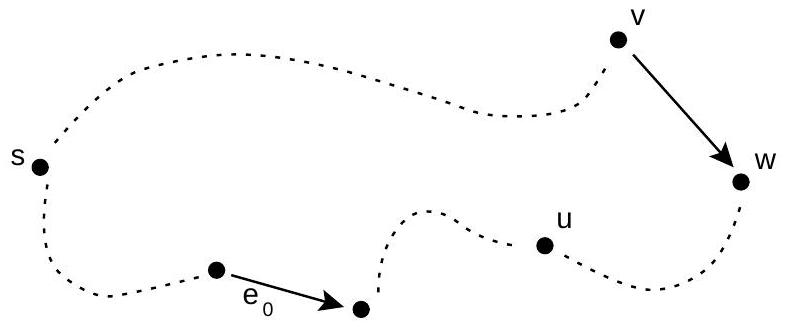
\includegraphics[max width=\textwidth, center]{2025_09_05_955b52bfc43174a24a9ag-24(2)}\\
y el camino en $T^{\prime}$ de $s$ a $u$ es el camino en $T$ de $s$ a $v$ seguido de la rama $(v, w)$ y seguido del camino en $T$ de $w$ a $u$. Luego, el camino en $T^{\prime}$ de $s$ a $u$ seguido del camino en $T$ de $s$ a $u$ recorrido en sentido inverso es el ciclo $\mathcal{C}$, de donde $y_{u}^{\prime}-y_{u}=c(\mathcal{C})=c_{v w}+y_{v}-y_{w}$, es decir, $y_{u}^{\prime}=y_{u}+c_{v w}+y_{v}-y_{w}$.\\
En cambio, si $v \notin R\left(T, e_{0}\right)$ entonces la situación es\\
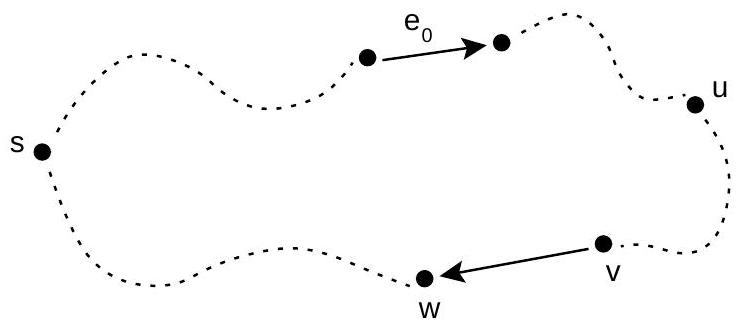
\includegraphics[max width=\textwidth, center]{2025_09_05_955b52bfc43174a24a9ag-24(1)}\\
y el camino en $T^{\prime}$ de $s$ a $u$ es el camino en $T$ de $s$ a $w$ seguido de la rama $(v, w)$ recorrida en sentido inverso y seguido del camino en $T$ de $v$ a $u$. Luego, el camino en $T$ de $s$ a $u$ seguido del camino en $T^{\prime}$ de $s$ a $u$ recorrido en sentido inverso es el ciclo $\mathcal{C}$, de donde $y_{u}-y_{u}^{\prime}=c(\mathcal{C})=c_{v w}+y_{v}-y_{w}$, es decir, $y_{u}^{\prime}=y_{u}-\left(c_{v w}+y_{v}-y_{w}\right)$.

\section*{Descripción del algoritmo.}
El algoritmo que describiremos sólo se podrá aplicar si conocemos una tree solution inicial y su correspondiente spanning tree. Veremos más adelante cómo encontrar una tree solution inicial que será lo análogo a la fase 1 (ver sección 8 del capítulo 1).\\
Fijemos un vértice $s$ de $G$. Sea $x$ una tree solution y sea $T$ un spanning tree tal que $x_{e}=0$ para todo $e \notin T$.

\begin{enumerate}
  \item Para cada $v \in V, v \neq s$ calcular el costo $y_{v}$ del único camino en $T$ de $s$ a $v, y_{s}=0$.
  \item Hallar $(v, w) \notin T$ tal que $c_{v w}+y_{v}-y_{w}<0$. Si no existe, STOP (en ese caso $x$ es óptimo, ver corolario 5.9.).
  \item Formar el circuito $\mathcal{C}$ agregando a $T$ la rama $(v, w)$. Si recorriendo $\mathcal{C}$ en el sentido de $(v, w)$ no hay ramas inversas STOP (en este caso no existe min $c x$, ver observación 5.10.).
  \item Calcular $\delta=\min \left\{x_{e} / e \in \mathcal{C}\right.$ es inversa $\}$.
  \item Si $e_{0} \in \mathcal{C}$ es una rama inversa tal que $\delta=x_{e_{0}}$, poner
\end{enumerate}

$$
y_{u}^{\prime}= \begin{cases}y_{u} & \text { si } u \in R\left(T, e_{0}\right) \\ y_{u}+c_{v w}+y_{v}-y_{w} & \text { si } u \notin R\left(T, e_{0}\right) \text { y } v \in R\left(T, e_{0}\right) \\ y_{u}-\left(c_{v w}+y_{v}-y_{w}\right) & \text { si } u \notin R\left(T, e_{0}\right) \text { y } v \notin R\left(T, e_{0}\right)\end{cases}
$$

\begin{enumerate}
  \setcounter{enumi}{5}
  \item Actualizar $x$ sumando $\delta$ al flujo de las ramas de $\mathcal{C}$ con la misma dirección de $(v, w)$ y restando $\delta$ al flujo de las ramas con dirección contraria a ( $v, w$ ). Actualizar $T$ reemplazándolo por el spanning tree que se obtiene agregándole la rama $(v, w)$ y quitándole la rama $e_{0}$ y actualizar $\left(y_{v}\right)$ poniendo $y_{v}=y_{v}^{\prime}$. GOTO 2.\\
Observación 5.10. Si no existe ninguna rama inversa en $\mathcal{C}$ entonces cualquiera sea $\mu>0$, si sumamos $\mu$ al flujo de todas las ramas de $\mathcal{C}$ obtendremos un nuevo flujo factible $x^{\prime}$ tal que $c x^{\prime}=c x+\mu c(\mathcal{C})$. Como $c(\mathcal{C})<0$ esto significa que no existe min $c x$.\\
Observación 5.11. Si al comenzar una iteración la tree solution $x$ presente en ese momento satisface $x_{e}>0$ para toda rama inversa $e \in \mathcal{C}$ (lo que ocurre, por ejemplo, si $x$ es una tree solution no degenerada) entonces $\delta>0$. En tal caso, la tree solution $x^{\prime}$ presente al comenzar la iteración siguiente que se obtiene sumando $\delta$ al flujo $x_{e}$ de las ramas $e \in \mathcal{C}$ con la misma dirección de $(v, w)$ y restando $\delta$ al flujo $x_{e}$ de las ramas $e$ con dirección contraria a $(v, w)$ satisface $c x^{\prime}=c x+\delta c(\mathcal{C})<c x$. Si esto ocurriera en cada iteración, entonces el algoritmo terminaría en un número finito de pasos ya que la cantidad de tree solutions es finita (ver corolario 5.5.). Pero si en alguna iteración la tree solution presente $x$ fuese degenerada entonces podría ocurrir que fuese $\delta=0$, y por lo tanto $c x=c x^{\prime}$. En este caso el algoritmo podría entrar en un loop. Sin embargo, tal como ocurre con el simplex, se puede modificar el algoritmo para que esto no ocurra. De esa manera, dado que hay finitas tree solutions, el algoritmo termina en un número finito de pasos. Para más detalles sobre este tema ver [Ahuja et al].
\end{enumerate}

\section*{6. La "FASE 1" para un grafo conexo.}
Para poder aplicar el algoritmo necesitamos conocer una tree solution inicial y su correspondiente spanning tree. Esto se logra de la siguiente manera: a partir del grafo $G=(V, E)$ creamos un nuevo grafo $G^{\prime}$ agregando a $G$ un nuevo vértice $\bar{s}$ que será la raíz, ramas ( $v, \bar{s}$ ) para cada $v \in V$ tal que $b_{v} \geq 0$ y ramas ( $\bar{s}, v$ ) para cada $v \in V$ tal que $b_{v}<0$ y tomemos $b_{\bar{s}}=0$. A las ramas que hemos agregado las llamaremos ramas artificiales. A las ramas de $e \in E$ les asignamos costo $c_{e}^{\prime}=0$ y a las ramas $e$ artificiales les asignamos costo $c_{e}^{\prime}=1$. Consideremos en $G^{\prime}$ el problema de flujo de mínimo costo


\begin{gather*}
\min c^{\prime} x \\
x(v, V \cup\{\bar{s}\})-x(V \cup\{\bar{s}\}, v)=b_{v} \quad \forall v \in V \cup\{\bar{s}\}  \tag{3}\\
x \geq 0
\end{gather*}


Observación 6.1. El flujo $x^{\prime}$ definido por

$$
x_{e}^{\prime}= \begin{cases}b_{v} & \text { si } b_{v} \geq 0 \text { y } e=(v, \bar{s}) \\ -b_{v} & \text { si } b_{v}<0 \text { y } e=(\bar{s}, v) \\ 0 & \text { si } e \in E\end{cases}
$$

es una tree solution para $G^{\prime}$. El correspondiente spanning tree es $T^{\prime}=\left(V^{\prime}, E^{\prime}\right)$, donde $V^{\prime}=V \cup\{\bar{s}\}$ y $E^{\prime}=\left\{(v, \bar{s}) / b_{v} \geq 0\right\} \cup\left\{(\bar{s}, v) / b_{v}<0\right\}$, ya que

$$
x^{\prime}(v, V \cup\{\bar{s}\})-x^{\prime}(V \cup\{\bar{s}\}, v)= \begin{cases}b_{v}-0=b_{v} & \text { si } v \neq \bar{s} \text { y } b_{v} \geq 0 \\ 0-\left(-b_{v}\right)=b_{v} & v \neq \bar{s} \text { y } b_{v}<0 \\ -\sum_{v \in V} b_{v}=0=b_{\bar{s}} & \text { si } v=\bar{s}\end{cases}
$$

y $x_{e}^{\prime}=0$ para todo $e \notin T^{\prime}$.\\
Luego, siempre podemos resolver (3) aplicando el algoritmo, utilizando la solución inicial $x^{\prime}$ y el correspondiente spanning tree $T^{\prime}$. Tal como ocurre en la fase 1 del algoritmo simplex visto en el capítulo 1 , la fase 1 de este algoritmo consiste en resolver (3) para hallar una tree solution inicial que nos permita aplicar el algoritmo para resolver (2).\\
Proposición 6.2. Se verifican\\
a) si (2) tiene alguna solución factible entonces (3) tiene una solución óptima $\bar{x}$ que verifica $c^{\prime} \bar{x}=0$ (y, por lo tanto, en cualquier solución óptima el valor del funcional será cero).\\
b) Si $\bar{x}$ es una tree solution óptima de (3) con spanning tree $T^{\prime}$, que verifica $c^{\prime} \bar{x}=0$ entonces el flujo $x$ definido por $x_{e}=\bar{x}_{e}$ para cada $e \in E$ es una tree solution para $G$. El correspondiente spanning tree $T$ se obtiene de $T^{\prime}$ de la siguiente manera:

\begin{enumerate}
  \item Sea $H$ el grafo que se obtiene eliminando en $T^{\prime}$ todas las ramas artificiales que contenga y el vértice $\bar{s}$.
  \item Elegir $v \in V$
  \item $A=\{v\}$
  \item Aplicar un algoritmo search para hallar todos los vértices $w$ tales que existe un camino en $H$ de $v$ a $w$.
  \item $A=A \cup\{w \in V / \exists$ un camino en $H$ de $v$ a $w\}$.
  \item Si $A=V$ STOP
  \item Elegir una rama $e \notin H$ de $G$ tal que uno de sus vértices pertenezca a $A$ y el otro no.
  \item Actualizar $H$ en la forma: $H=$ grafo obtenido agregando $e$ a $H$.
  \item GOTO 4.
\end{enumerate}

Demostración: a) Si (2) tiene una solución factible $x$ entonces el flujo $\bar{x}$ definido por

$$
\bar{x}_{e}= \begin{cases}x_{e} & \text { si } e \in E \\ 0 & \text { si } e \text { es una rama artificial }\end{cases}
$$

es una solución factible de (3) que verifica $c^{\prime} \bar{x}=0$. Pero como el valor del funcional en cualquier solución factible de (3) es mayor o igual que cero (pues el costo de las ramas es 0 o 1 y el flujo es no negativo) entonces $\bar{x}$ es una solución óptima que satisface $c^{\prime} \bar{x}=0$.\\
b) Si $\bar{x}$ es una tree solution óptima de (3) con spanning tree $T^{\prime}$ que verifica $c^{\prime} \bar{x}=0$ entonces debe ser $\bar{x}_{e}=0$ para toda rama artificial $e$ pues por la forma en que definimos $c^{\prime}$ resulta que $c^{\prime} \bar{x}=\sum_{\text {eartificial }} \bar{x}_{e}$ y por lo tanto si fuese $\bar{x}_{e}>0$ para alguna rama artificial entonces resultaría que $c^{\prime} \bar{x}>0$.\\
Luego, $x$ es una solución factible de (2) y las ramas que tienen flujo no nulo pertenecen al grafo que se obtiene eliminando en $T^{\prime}$ las ramas artificiales que contenga y el vértice $\bar{s}$.\\
Veamos ahora que el algoritmo definido por los pasos 1. a 9 . nos da un spanning tree $T$ de $G$ tal que $x_{e}=0$ para toda $e \notin T$.

Primero observemos que al quitar las ramas artificiales de $T^{\prime}$ el grafo $H$ resultante tiene como vértices a todos los vértices de $G$ y es acíclico (ya que es un subgrafo de un spanning tree), pero el problema es que podría no ser conexo.

En cada iteración, el conjunto $A$ que vamos formando es el conjunto de todos los vértices de $G$ que están en la misma componente conexa que $v$ del presente $H$. Además, en cada iteración el grafo $H$ es acíclico pues lo es el $H$ inicial y cada rama que agregamos no forma ciclo con las del presente $H$ : en efecto, las ramas que se agregan tienen un vértice $u \in A$ otro vértice $w \notin A$. Luego, si al agregar esa rama se formara un ciclo entonces existiría en $H$ un camino de $u$ a $w$. Pero como $u \in A$ entonces existe un camino de $v$ a $u$ el cual, seguido del camino de $u$ a $w$ nos daría un camino de $v$ a $w$ lo que contradice que $w \notin A$. Luego, cuando $A=V$ el grafo $T=H$ que se tiene en ese momento es conexo y acíclico y como partimos de un grafo cuyos vértices son todos los vértices de $G$ entonces es un spanning tree de $G$ y como las ramas que tenían flujo no nulo pertenecían al $H$ inicial entonces $x_{e}=0$ para todo $e \notin T$, lo que muestra que $x$ es una tree solution con spanning tree $T$.

Finalmente observemos que si $A \neq V$ entonces el paso 7. siempre se puede realizar. En efecto, sea $w$ tal que $w \notin A$. Como $G$ es conexo, sea $\mathcal{P}$ un camino en $G$ de $v$ a $w$. Entonces, como $v \in A$ y $w \notin A$ alguna rama $e$ de ese camino tiene un extremo en $A$ y el otro en $V-A$ : sea $\mathcal{P}$ el camino\\
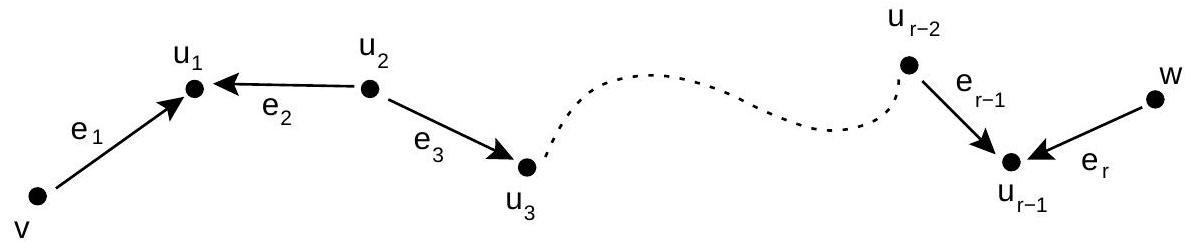
\includegraphics[max width=\textwidth, center]{2025_09_05_955b52bfc43174a24a9ag-27}\\
si $u_{1} \notin A$ entonces basta tomar $e=e_{1}$ pues $v \in A$, si $u_{1} \in A$ y $u_{2} \notin A$ entonces basta tomar $e=e_{2}, \ldots$, si $u_{r-2} \in A$ y $u_{r-1} \notin A$ entonces basta tomar $e=e_{r-1}$ y si $u_{r-1} \in A$ entonces basta tomar $e=e_{r}$ pues $w \notin A$. $\square$

Luego, la fase 1 puede describirse como sigue: aplicamos el algoritmo para resolver (3) tomando como tree solution inicial la definida en la observación 6.1.\\
Si al terminar el algoritmo obtenemos una tree solution óptima de (3) $\bar{x}$ con spanning tree $T^{\prime}$, que verifica $c^{\prime} \bar{x}=0$ entonces obtenemos una tree solution $x$ para $G$ y su correspondiente spanning tree en la forma descripta en la proposición 6.2. y volvemos a aplicar el algoritmo, ahora para resolver (2) utilizando $x$ como tree solution inicial. En caso contrario el problema no tiene soluciones factibles.

\section*{7. Algoritmo "simplex" para el problema del transporte.}
Por razones de claridad aplicaremos el algoritmo en un ejemplo particular, pero el lector se dará cuenta de que este procedimiento puede aplicarse en cualquier caso.\\
Supongamos que tenemos tres depósitos y cuatro clientes y queremos determinar la manera más barata de transportar cierta mercadería de los depósitos a los clientes. Si el costo $c_{i j}$ de transportar una unidad de mercadería desde el depósito $v_{i}(1 \leq i \leq 3)$ al cliente $w_{j}(1 \leq j \leq 4)$ está dado por la matriz

$$
C=\left(c_{i j}\right)=\left(\begin{array}{cccc}
8 & 6 & 10 & 9 \\
9 & 12 & 13 & 7 \\
14 & 9 & 16 & 5
\end{array}\right),
$$

las cantidades ofrecidas por los depósitos son $b_{v_{1}}=35, b_{v_{2}}=50$ y $b_{v_{3}}=40$ respectivamente y las demandadas por los clientes son $-b_{w_{1}}=45,-b_{w_{2}}=20,-b_{w_{3}}=30 \mathrm{y}-b_{w_{4}}=30$ respectivamente, llamando $x_{i j}$ a la\\
cantidad de unidades que se transportan del depósito $v_{i}$ al cliente $w_{j}$ el problema puede plantearse en la forma

$$
\begin{aligned}
& \min \sum_{i j} c_{i j} x_{i j} \\
& \sum_{j} x_{i j} \leq b_{v_{i}} \\
& \sum_{i} x_{i j}=-b_{w_{j}} \\
& x_{i j} \geq 0
\end{aligned}
$$

Tal como vimos en el capítulo anterior, agregando un cliente de ser necesario, podemos suponer que la primera ecuación de las restricciones es una igualdad. Luego podemos suponer que las restricciones son

$$
\begin{aligned}
\sum_{j} x_{i j} & =b_{v_{i}} \\
-\sum_{i} x_{i j} & =b_{w_{j}} \\
x_{i j} & \geq 0
\end{aligned}
$$

Esta situación puede ser representada en el grafo bipartito $G=(V, E)$ donde

$$
V=\left\{v_{1}, v_{2}, v_{3}\right\} \cup\left\{w_{1}, w_{2}, w_{3}, w_{4}\right\}
$$

y

$$
E=\left\{\left(v_{i}, w_{j}\right) / 1 \leq i \leq 3,1 \leq j \leq 4\right\}
$$

es decir, el grafo\\
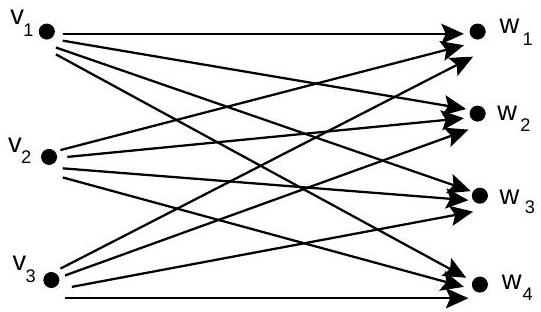
\includegraphics[max width=\textwidth, center]{2025_09_05_955b52bfc43174a24a9ag-28}\\
y pensando a $x_{i j}$ como el flujo de la rama ( $v_{i}, w_{j}$ ) el problema se escribe

$$
\begin{gathered}
\min c x \\
x(v, V)-x(V, v)=b_{v} \quad \forall v \in V \\
x_{e} \geq 0 \quad \forall e \in E
\end{gathered}
$$

El siguiente procedimiento, conocido como la regla del noroeste nos permite hallar una tree solution inicial evitando la fase 1.\\
Consideremos la matriz

$$
\left(x_{i j}\right)=\left(\begin{array}{llll}
x_{11} & x_{12} & x_{13} & x_{14} \\
x_{21} & x_{22} & x_{23} & x_{24} \\
x_{31} & x_{32} & x_{33} & x_{34}
\end{array}\right)
$$

Queremos darle valores no negativos a $x_{i j}$ de manera que la suma de los coeficientes de la $i$-ésima fila sea $b_{v_{i}}$ y la suma de los de la $j$-ésima columna sea $-b_{w_{j}}$. El procedimiento es el siguiente:

\begin{enumerate}
  \item Ponemos $F_{i}=b_{v_{i}}(1 \leq i \leq 3), C_{j}=-b_{w_{j}}(1 \leq j \leq 4)$.
  \item Consideremos la submatriz $U$ de $\left(x_{i j}\right)$ formada por las filas y columnas que todavía no han sido fijadas.
  \item Sea $x_{r s}$ el coeficiente de $U$ que se encuentra más al noroeste. Entonces actualizamos ( $x_{i j}$ ) poniendo $x_{r s}=\min \left\{F_{r}, C_{s}\right\}$. Si $\min \left\{F_{r}, C_{s}\right\}=F_{r}$ también ponemos $x_{r j}=0$ para todo $x_{r j}$ que aún no tenga valor asignado. En caso contrario, ponemos $x_{i s}=0$ para todo $x_{i s}$ que aún no tenga valor asignado.
  \item Actualizamos $F_{r}$ y $C_{s}$ en la forma $F_{r}=F_{r}-x_{r s}, C_{s}=C_{s}-x_{r s}$. Si $F_{i}=0=C_{j}$ para todo $i, j$ STOP. En caso contrario, GOTO 2.\\
Aplicando esto a nuestro ejemplo obtenemos:
  \item $F_{1}=35, F_{2}=50, F_{3}=40, C_{1}=45, C_{2}=20, C_{3}=30, C_{4}=30$
  \item 
\end{enumerate}

$$
U=\left(\begin{array}{llll}
x_{11} & x_{12} & x_{13} & x_{14} \\
x_{21} & x_{22} & x_{23} & x_{24} \\
x_{31} & x_{32} & x_{33} & x_{34}
\end{array}\right)
$$

\begin{enumerate}
  \setcounter{enumi}{2}
  \item $r=s=1$. Ponemos $x_{11}=\min \left\{F_{1}, C_{1}\right\}=F_{1}=35$ y $x_{1 j}=0$ para todo $j \neq 1$. Ahora
\end{enumerate}

$$
\left(x_{i j}\right)=\left(\begin{array}{cccc}
35 & 0 & 0 & 0 \\
x_{21} & x_{22} & x_{23} & x_{24} \\
x_{31} & x_{32} & x_{33} & x_{34}
\end{array}\right)
$$

\begin{enumerate}
  \setcounter{enumi}{3}
  \item $F_{1}=0, F_{2}=50, F_{3}=40, C_{1}=10, C_{2}=20, C_{3}=30, C_{4}=30$
  \item Ahora
\end{enumerate}

$$
U=\left(\begin{array}{llll}
x_{21} & x_{22} & x_{23} & x_{24} \\
x_{31} & x_{32} & x_{33} & x_{34}
\end{array}\right)
$$

\begin{enumerate}
  \setcounter{enumi}{2}
  \item $r=2, s=1$. Ponemos $x_{21}=\min \left\{F_{2}, C_{1}\right\}=C_{1}=10$ y $x_{i 1}=0$ para todo $x_{i 1}$ que no tenga valor asignado. Ahora
\end{enumerate}

$$
\left(x_{i j}\right)=\left(\begin{array}{cccc}
35 & 0 & 0 & 0 \\
10 & x_{22} & x_{23} & x_{24} \\
0 & x_{32} & x_{33} & x_{34}
\end{array}\right)
$$

\begin{enumerate}
  \setcounter{enumi}{3}
  \item $F_{1}=0, F_{2}=40, F_{3}=40, C_{1}=0, C_{2}=20, C_{3}=30, C_{4}=30$
  \item Ahora
\end{enumerate}

$$
U=\left(\begin{array}{lll}
x_{22} & x_{23} & x_{24} \\
x_{32} & x_{33} & x_{34}
\end{array}\right)
$$

\begin{enumerate}
  \setcounter{enumi}{2}
  \item $r=2, s=2$. Ponemos $x_{22}=\min \left\{F_{2}, C_{2}\right\}=C_{2}=20$ y $x_{i 2}=0$ para todo $x_{i 2}$ que no tenga valor asignado. Ahora
\end{enumerate}

$$
\left(x_{i j}\right)=\left(\begin{array}{cccc}
35 & 0 & 0 & 0 \\
10 & 20 & x_{23} & x_{24} \\
0 & 0 & x_{33} & x_{34}
\end{array}\right)
$$

\begin{enumerate}
  \setcounter{enumi}{3}
  \item $F_{1}=0, F_{2}=20, F_{3}=40, C_{1}=0, C_{2}=0, C_{3}=30, C_{4}=30$
  \item Ahora $U=\left(\begin{array}{ll}x_{23} & x_{24} \\ x_{33} & x_{34}\end{array}\right)$
  \item $r=2, s=3$. Ponemos $x_{23}=\min \left\{F_{2}, C_{3}\right\}=F_{2}=20$ y $x_{2 j}=0$ para todo $x_{2 j}$ que no tenga valor asignado. Ahora
\end{enumerate}

$$
\left(x_{i j}\right)=\left(\begin{array}{cccc}
35 & 0 & 0 & 0 \\
10 & 20 & 20 & 0 \\
0 & 0 & x_{33} & x_{34}
\end{array}\right)
$$

\begin{enumerate}
  \setcounter{enumi}{3}
  \item $F_{1}=0, F_{2}=0, F_{3}=40, C_{1}=0, C_{2}=0, C_{3}=10, C_{4}=30$
  \item Ahora $U=\left(\begin{array}{ll}x_{33} & x_{34}\end{array}\right)$
  \item $r=3, s=3$. Ponemos $x_{33}=\min \left\{F_{3}, C_{3}\right\}=C_{3}=10$ y $x_{i 3}=0$ para todo $x_{i 3}$ que no tenga valor asignado. Ahora
\end{enumerate}

$$
\left(x_{i j}\right)=\left(\begin{array}{cccc}
35 & 0 & 0 & 0 \\
10 & 20 & 20 & 0 \\
0 & 0 & 10 & x_{34}
\end{array}\right)
$$

\begin{enumerate}
  \setcounter{enumi}{3}
  \item $F_{1}=0, F_{2}=0, F_{3}=30, C_{1}=0, C_{2}=0, C_{3}=0, C_{4}=30$
  \item Ahora $U=\left(x_{34}\right)$
  \item $r=3, s=4$. Ponemos $x_{34}=\min \left\{F_{3}, C_{4}\right\}=F_{3}=30$ y $x_{3 j}=0$ para todo $x_{3 j}$ que no tenga valor asignado. Ahora
\end{enumerate}

$$
\left(x_{i j}\right)=\left(\begin{array}{cccc}
35 & 0 & 0 & 0 \\
10 & 20 & 20 & 0 \\
0 & 0 & 10 & 30
\end{array}\right)
$$

\begin{enumerate}
  \setcounter{enumi}{3}
  \item $F_{1}=0, F_{2}=0, F_{3}=0, C_{1}=0, C_{2}=0, C_{3}=0, C_{4}=0$
\end{enumerate}

De esta manera obtenemos la tree solution inicial\\
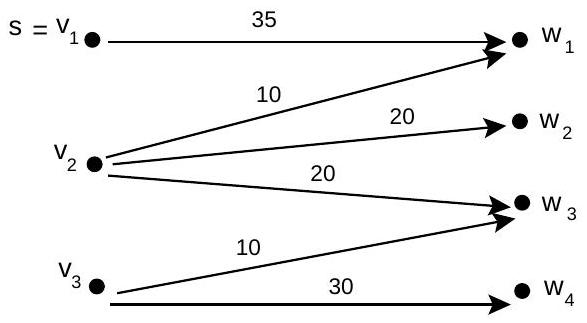
\includegraphics[max width=\textwidth, center]{2025_09_05_955b52bfc43174a24a9ag-30}\\
donde en cada rama hemos indicado el valor de su flujo. Elijamos cualquier vértice como raíz $s$ de este spanning tree $T$, por ejemplo $s=v_{1}$. Ahora pongamos $y_{s}=0$ y calculemos $y_{u}$ para cada $u \neq s$. Por el corolario 5.9. para cada $i, j$ tal que $\left(v_{i}, w_{j}\right) \in T$ se verifica $c_{i j}+y_{v_{i}}-y_{w_{j}}=0$ y además $0=y_{s}=y_{v_{1}}$. Luego, $\left(y_{u}\right)_{u \in V}$ debe ser solución del sistema

$$
\begin{aligned}
y_{w_{j}}-y_{v_{i}} & =c_{i j} \quad\left(v_{i}, w_{j}\right) \in T \\
y_{v_{1}} & =0
\end{aligned}
$$

Este sistema tiene 7 ecuaciones y 7 incógnitas y tiene solución única ya que fijados $T$ y $s$ hay un único camino de $s$ a $u$ para todo $u \neq s$. Además, este sistema puede resolverse fácilmente por sustitución. En efecto, el sistema es

$$
\begin{aligned}
y_{w_{1}}-y_{v_{1}} & =8 \\
y_{w_{1}}-y_{v_{2}} & =9 \\
y_{w_{2}}-y_{v_{2}} & =12 \\
y_{w_{3}}-y_{v_{2}} & =13 \\
y_{w_{3}}-y_{v_{3}} & =16 \\
y_{w_{4}}-y_{v_{3}} & =5 \\
y_{v_{1}} & =0
\end{aligned}
$$

Como por la última ecuación $y_{v_{1}}=0$ entonces de la primera resulta que $y_{w_{1}}=8$, de la segunda que $y_{v_{2}}=-1$, de la tercera y cuarta que $y_{w_{2}}=11, y_{w_{3}}=12$, de la quinta que $y_{v_{3}}=-4$ y de la sexta que $y_{w_{4}}=1$.\\
Ahora calculemos $\bar{c}_{i j}=c_{i j}+y_{v_{i}}-y_{w_{j}}$. para $i, j$ tal que $\left(v_{i}, w_{j}\right) \notin T$. Dejamos a cargo del lector verificar que $\bar{c}_{12}=-5, \bar{c}_{13}=-2, \bar{c}_{14}=8, \bar{c}_{24}=5, \bar{c}_{31}=2, \bar{c}_{32}=-6$.\\
Elegimos $e \notin T$ tal que $c_{e}<0$. Por ejemplo, $e=\left(v_{3}, w_{2}\right)$ y formemos el circuito $\mathcal{C}$ que resulta agregando $e$ a $T$. Recorriendo $\mathcal{C}$ en el sentido de $e=\left(v_{3}, w_{2}\right)$ las ramas inversas son ( $v_{2}, w_{2}$ ) con flujo $x_{22}=20$ y ( $v_{3}, w_{3}$ ) con flujo $x_{33}=10$. Ahora actualizamos el flujo sumando $\delta=\min \left\{x_{e} / e \in \mathcal{C}\right.$ es inversa $\}=10$ al flujo de las ramas directas y restando $\delta$ al flujo de las ramas inversas de $\mathcal{C}$ y luego eliminamos de $T$ la rama ( $v_{3}, w_{3}$ ) que ahora tiene flujo nulo y le agregamos la rama ( $v_{3}, w_{2}$ ). De esta manera obtenemos la nueva tree solution\\
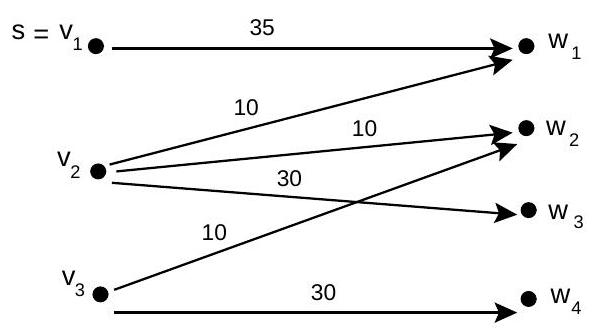
\includegraphics[max width=\textwidth, center]{2025_09_05_955b52bfc43174a24a9ag-31}

Dejamos a cargo del lector el cálculo de los nuevos valores de ( $y_{u}$ ) y verificar que los nuevos $\bar{c}_{i j}$ son $\bar{c}_{12}=-5$, $\bar{c}_{13}=-2, \bar{c}_{14}=2, \bar{c}_{24}=-1, \bar{c}_{31}=8, \bar{c}_{33}=6$.\\
Ahora elegimos $e \notin T$ tal que $c_{e}<0$, por ejemplo, $e=\left(v_{1}, w_{2}\right)$ y repitiendo el procedimiento anterior (en este caso $\delta=10$, la rama que se elimina es ( $v_{2}, w_{2}$ ) y la que se agrega es ( $v_{1}, w_{2}$ )) obtenemos la nueva tree solution\\
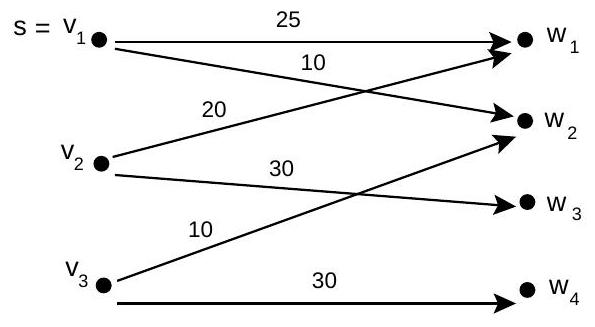
\includegraphics[max width=\textwidth, center]{2025_09_05_955b52bfc43174a24a9ag-31(2)}

Nuevamente dejamos a cargo del lector la actualización de $\left(y_{u}\right)$ y verificar que los nuevos valores de $\bar{c}_{i j}$ son $\bar{c}_{13}=-2, \bar{c}_{14}=7, \bar{c}_{22}=5, \bar{c}_{24}=4, \bar{c}_{31}=3, \bar{c}_{33}=1$.\\
Eligiendo ahora $e=\left(v_{1}, w_{3}\right)$ y repitiendo el procedimiento (ahora $\delta=25$, la rama que se elimina es ( $v_{1}, w_{1}$ ) y la que se agrega es $\left.\left(v_{1}, w_{3}\right)\right)$ se obtiene la tree solution\\
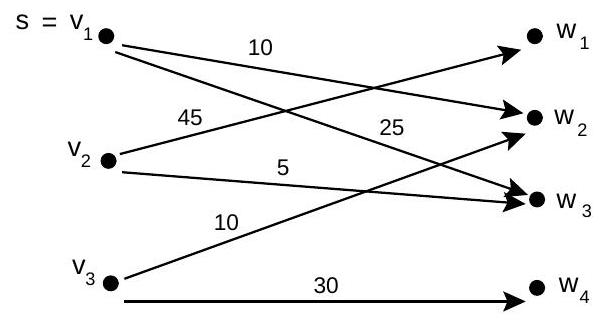
\includegraphics[max width=\textwidth, center]{2025_09_05_955b52bfc43174a24a9ag-31(1)}\\
que resulta ser óptima ya que $\bar{c}_{i j} \geq 0$ para todo $i, j$ tal que $\left(v_{i}, w_{j}\right) \notin T$.\\
En este ejemplo hemos usado el hecho de que si $T$ es un spanning tree de un grafo conexo $G$ entonces el sistema

$$
y_{w}-y_{v}=c_{v w} \quad(v, w) \in T
$$

con $m-1$ ecuaciones y $m$ incógnitas (donde $m$ es la cantidad de vértices de $G$ ) tiene rango $m-1$ y se puede resover dándole un valor arbitrario (en nuestro caso cero) a una indeterminada y obteniendo las restantes por sustitución. Veremos ahora que este hecho vale en general.

Proposición 7.1. Sea $A$ la matriz de incidencia vértice-rama de un grafo conexo $G$ con $m$ vértices y sea $B \in \mathbb{R}^{m \times(m-1)}$ la submatriz de $A$ formada por las columnas de $A$ que corresponden a las ramas de un spanning tree $T$ de $G$. Entonces existe una matriz $B^{\prime}$ obtenida permutando algunas filas y columnas de $B$ tal que $B^{\prime}$ es triangular y vale $\operatorname{rg} A=\operatorname{rg} B=\operatorname{rg} B^{\prime}=m-1$.\\
Demostración: Como $T$ es un árbol entonces tiene al menos una hoja $u$ y sea $e$ la única rama que incide en $u$. Luego, en la fila $u, B$ tiene una única componente no nula, en la columna $e$, que vale $10-1$.

Intercambiando si es necesario una fila y una columna de $B$ obtenemos

$$
B_{1}^{\prime}=\left(\begin{array}{cccc} 
& & & * \\
& B_{1} & & \vdots \\
& & & * \\
0 & \cdots & 0 & \pm 1
\end{array}\right)
$$

donde $B_{1}^{\prime}$ es la matriz de incidencia del árbol que resulta de suprimir en $T$ la hoja $u$ y la rama $e$. Luego, $B_{1}$ es una matriz de incidencia vértice-rama de un árbol y podemos repetir el procedimiento con $B_{1}$. Permutando si es necesario una fila y una columna de $B_{1}$ podemos obtener la matriz

$$
\left(\begin{array}{cccc} 
& & & * \\
& B_{2} & & \vdots \\
& & & * \\
0 & \cdots & 0 & \pm 1
\end{array}\right)
$$

y permutando esas mismas filas y columnas en $B_{1}^{\prime}$ obtenemos

$$
B_{2}^{\prime}=\left(\begin{array}{ccccc} 
& & & * & * \\
& B_{1} & & \vdots & \vdots \\
& & & * & * \\
0 & \cdots & 0 & \pm 1 & * \\
0 & \cdots & 0 & 0 & \pm 1
\end{array}\right)
$$

Repitiendo este procedimiento finalmente obtenemos

$$
B^{\prime}=\left(\begin{array}{ccccccc} 
\pm 1 & * & * & * & \cdots & * & * \\
\pm 1 & * & * & * & \cdots & * & * \\
0 & \pm 1 & * & * & \cdots & * & * \\
0 & 0 & \pm 1 & * & \cdots & * & * \\
\vdots & \vdots & \vdots & \vdots & \vdots & \vdots & \vdots \\
0 & 0 & 0 & 0 & \cdots & 0 & \pm 1
\end{array}\right)
$$

Como $B^{\prime}$ se obtuvo permutando filas y columnas de $B$ entonces $\operatorname{rg} B=\operatorname{rg} B^{\prime}=m-1$. Además, como las columnas de $B$ son algunas de las columnas de $A$ entonces debe ser $\operatorname{rg} A \geq \operatorname{rg} B=m-1$. Pero por otra parte, como $A$ tiene $m$ filas y la suma de ellas es cero (por ser la matriz de incidencia de un grafo, ver observación 1.13. del capítulo 2) entonces $\operatorname{rg} A<m$, de donde $\operatorname{rg} A=m-1$. ㅁ

Corolario 7.2. Con las mismas hipótesis de la proposición anterior, el sistema $y \cdot B=c$ se puede resolver dándole a una indeterminada un valor arbitrario y obteniendo las restantes por sustitución.


\end{document}